\documentclass{article}

% Language setting
% Replace `english' with e.g. `spanish' to change the document language
\usepackage[english]{babel}

% Set page size and margins
% Replace `letterpaper' with `a4paper' for UK/EU standard size
\usepackage[letterpaper,top=2cm,bottom=2cm,left=3cm,right=3cm,marginparwidth=1.75cm]{geometry}

% Useful packages
\usepackage{amsmath}
\usepackage{graphicx}
\usepackage[colorlinks=true, allcolors=blue]{hyperref}
\usepackage{float}

\title{CS460: Assignment 3}
\author{Arya Shetty || Damon Lin}
\begin{document}
\maketitle

\section{Potential Functions}
All animation gifs are in the folders labeled the same as the pictures here.

This program addressed creating a potential function path planner for a rigid body robot that could only translate and not rotate. For the attractive potential gradient of the function, we implemented a force that was proportional to the difference between the current position of the robot and the goal. This meant that as the robot moved farther from the goal, the force got larger, and the closer it would be, the more it would be able to guide the robot. For the repulsive gradient, we used the distance from the robot to an obstacle in the environment. If this distance is larger than a set threshold we define then we don't factor in the repulsive force, if it is that means it's crossed the minimum safe distance and must repel from the obstacle. To calculate the gradient, the function uses central differences, which estimate the gradient based on how much the distance changes when you move the robot in the x and y directions. We use a small epsilon to perturb the robot in both the positive and negative directions and get new distances. We then multiply this by the inversely proportional force (1/d), which creates a stronger repulsive force if the robot is closer to the obstacle. The returned gradient is negative since we want the robot to move away. Next, we can calculate the total gradient, and we normalize it if it's too large to avoid overshooting and not moving too quickly. I reused the distance to the obstacle, got rotated vertices, and loaded obstacles from previous codes. For the actual planning, we use gradient descent from algorithm 1 over a set amount of iterations and save the path to then animate. Below, you will see the five environments from the previous assignment and 5 different paths for each one using the potential function planner. We set the attractive, repulsive, and radius constants the same for all the tests to keep it fair (0.5, 200, 0.25). The successes, failures, and path lengths are posted below. The five starts and goals:\newline
(0,0) (3,2.5) \newline
(10,1) (5,5) \newline
(0,0) (10,10) \newline
(10,1) (18,17) \newline
(0,0) (5,15)\newline
In terms of the results, they were mostly successful, especially due to the radius constant being small, so it could fit through tight gaps, which is usually a problem for potential functions. It failed only where the goal was too close to the obstacle making the forces impossible to push the robot there.

\begin{figure} [H]
    \centering
    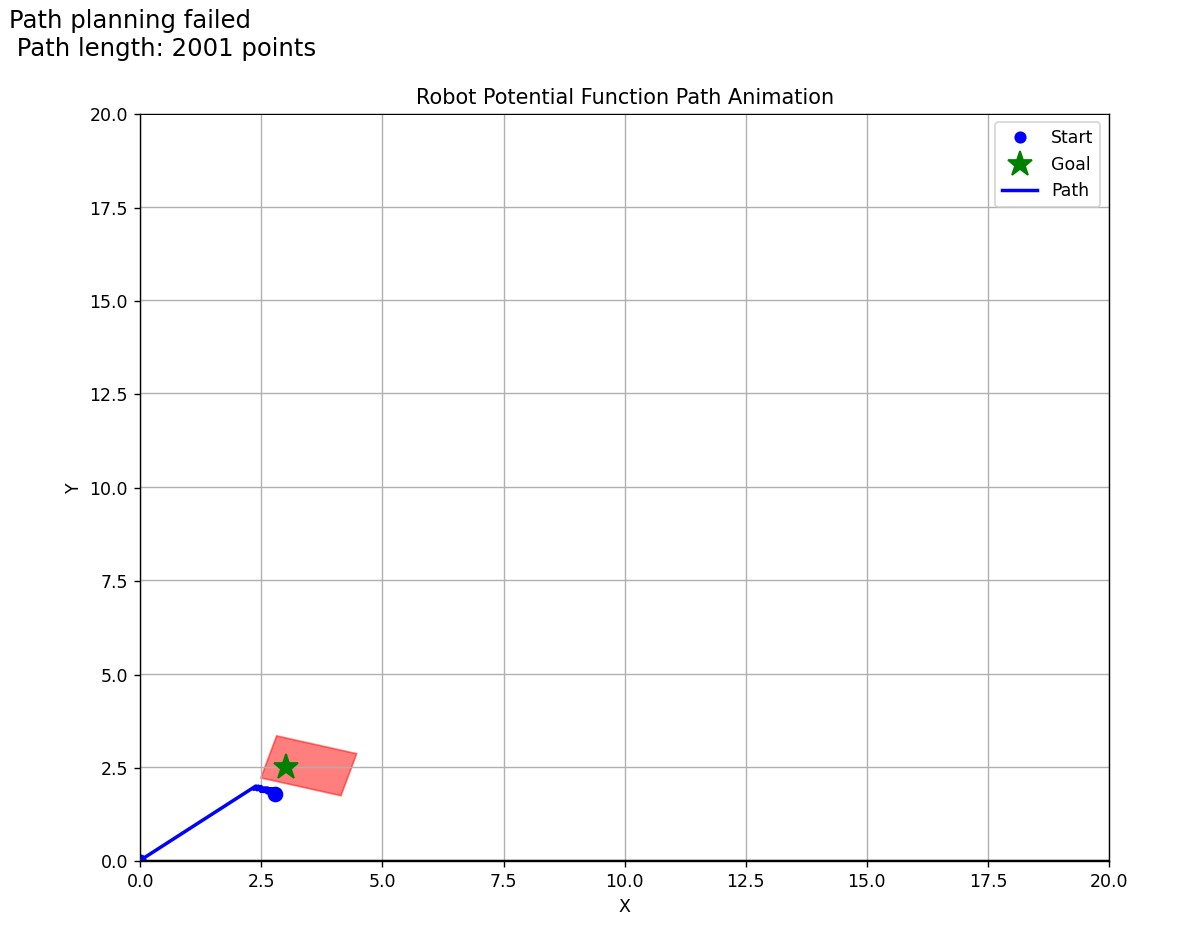
\includegraphics[width=0.5\linewidth]{latex_media/Env1PotentialTest1.jpg}
    \caption{Environment 1 Potential Test 1 (Fail)}
\end{figure}

\begin{figure} [H]
    \centering
    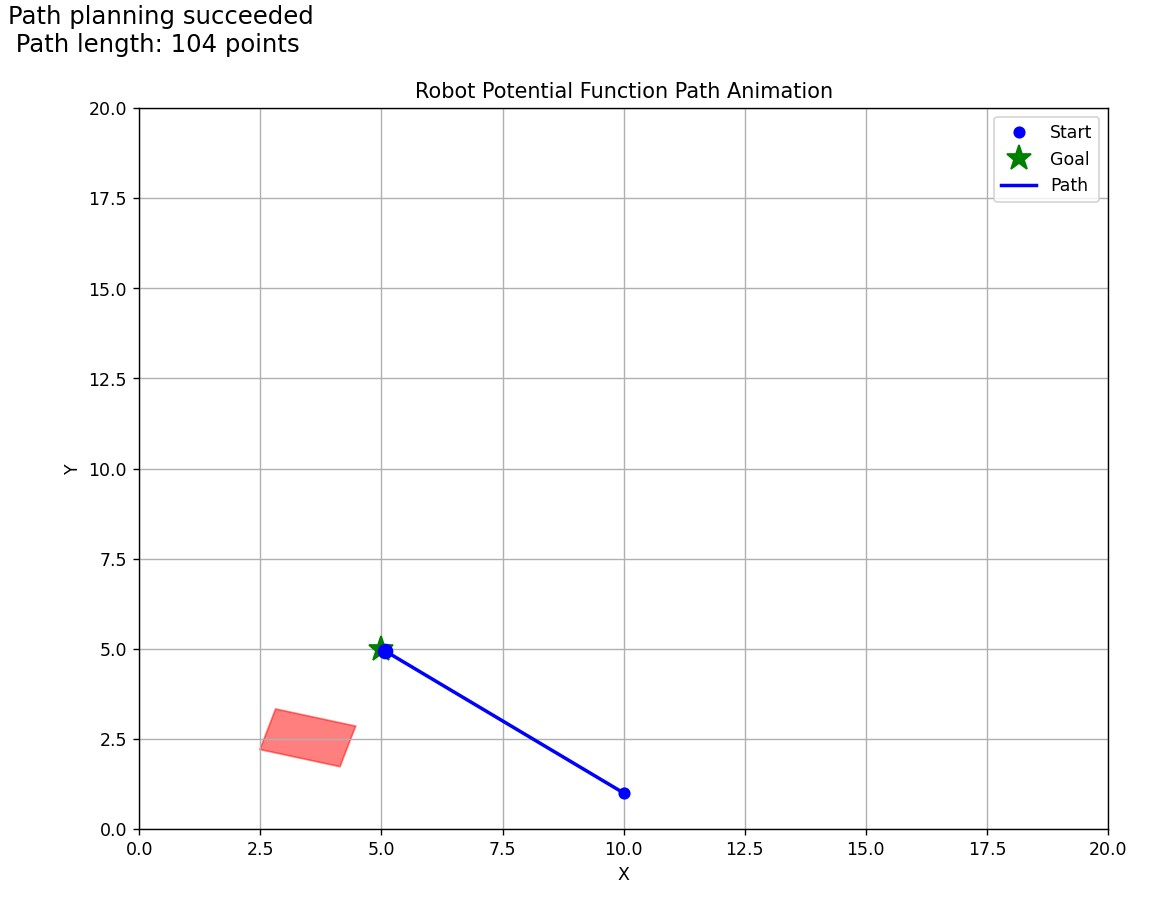
\includegraphics[width=0.5\linewidth]{latex_media/Env1PotentialTest2.jpg}
    \caption{Environment 1 Potential Test 2}
\end{figure}

\begin{figure} [H]
    \centering
    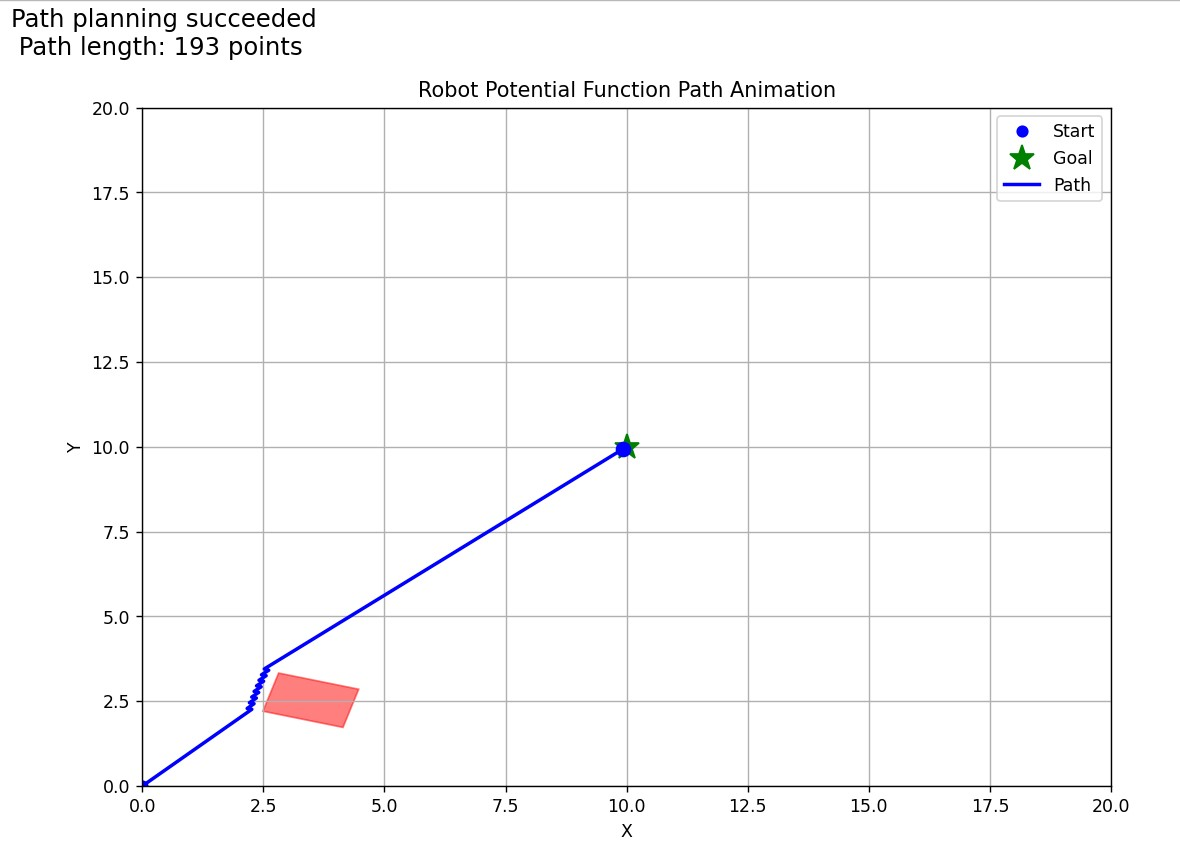
\includegraphics[width=0.5\linewidth]{latex_media/Env1PotentialTest3.jpg}
    \caption{Environment 1 Potential Test 3}
\end{figure}

\begin{figure} [H]
    \centering
    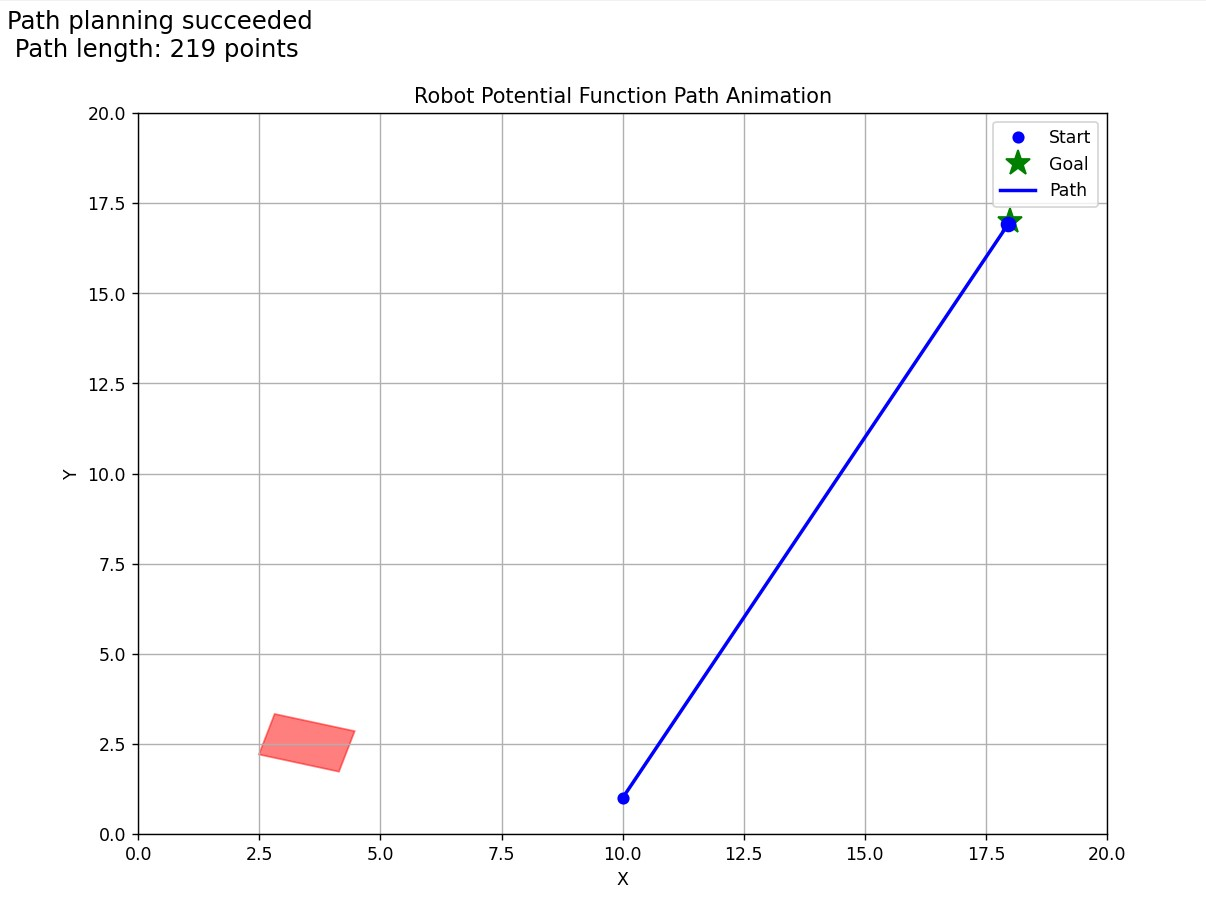
\includegraphics[width=0.5\linewidth]{latex_media/Env1PotentialTest4.jpg}
    \caption{Environment 1 Potential Test 4}
\end{figure}

\begin{figure} [H]
    \centering
    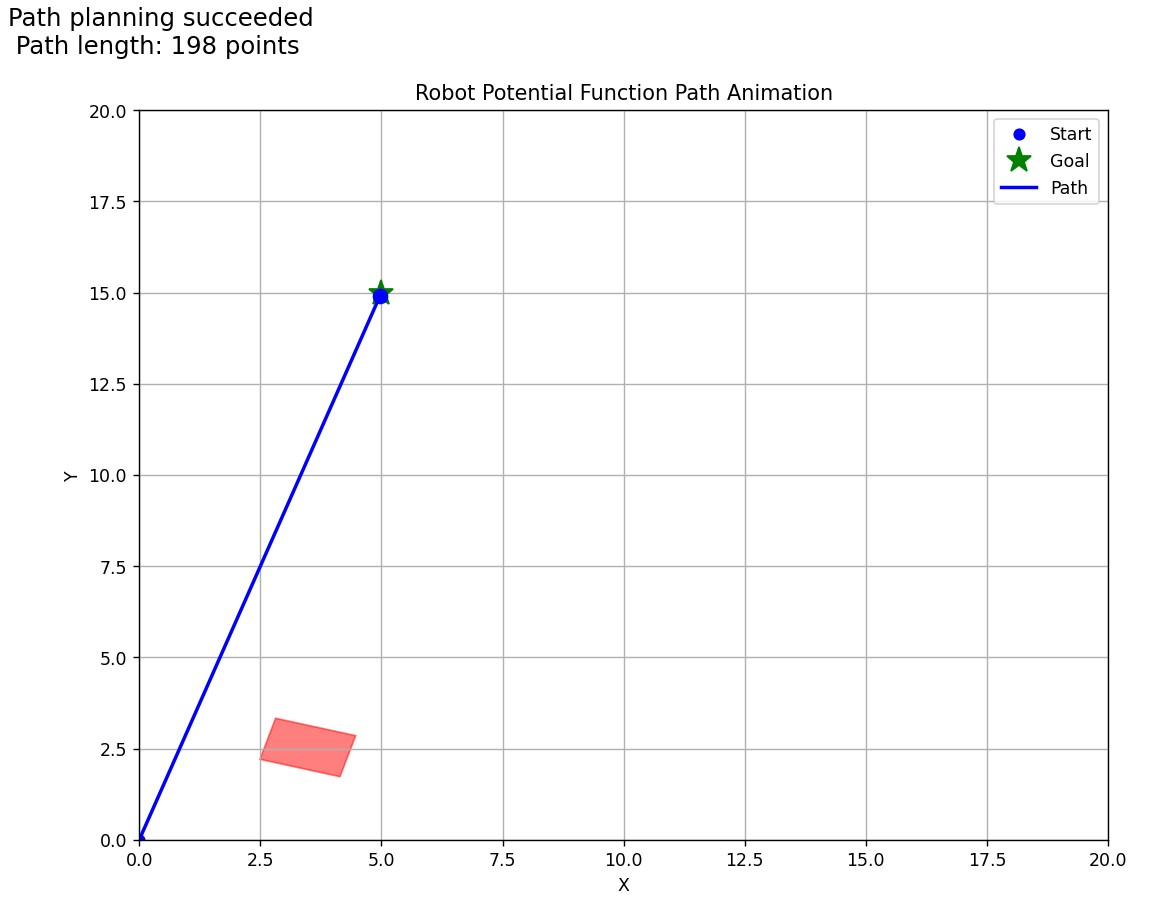
\includegraphics[width=0.5\linewidth]{latex_media/Env1PotentialTest5.jpg}
    \caption{Environment 1 Potential Test 5}
\end{figure}

\begin{figure} [H]
    \centering
    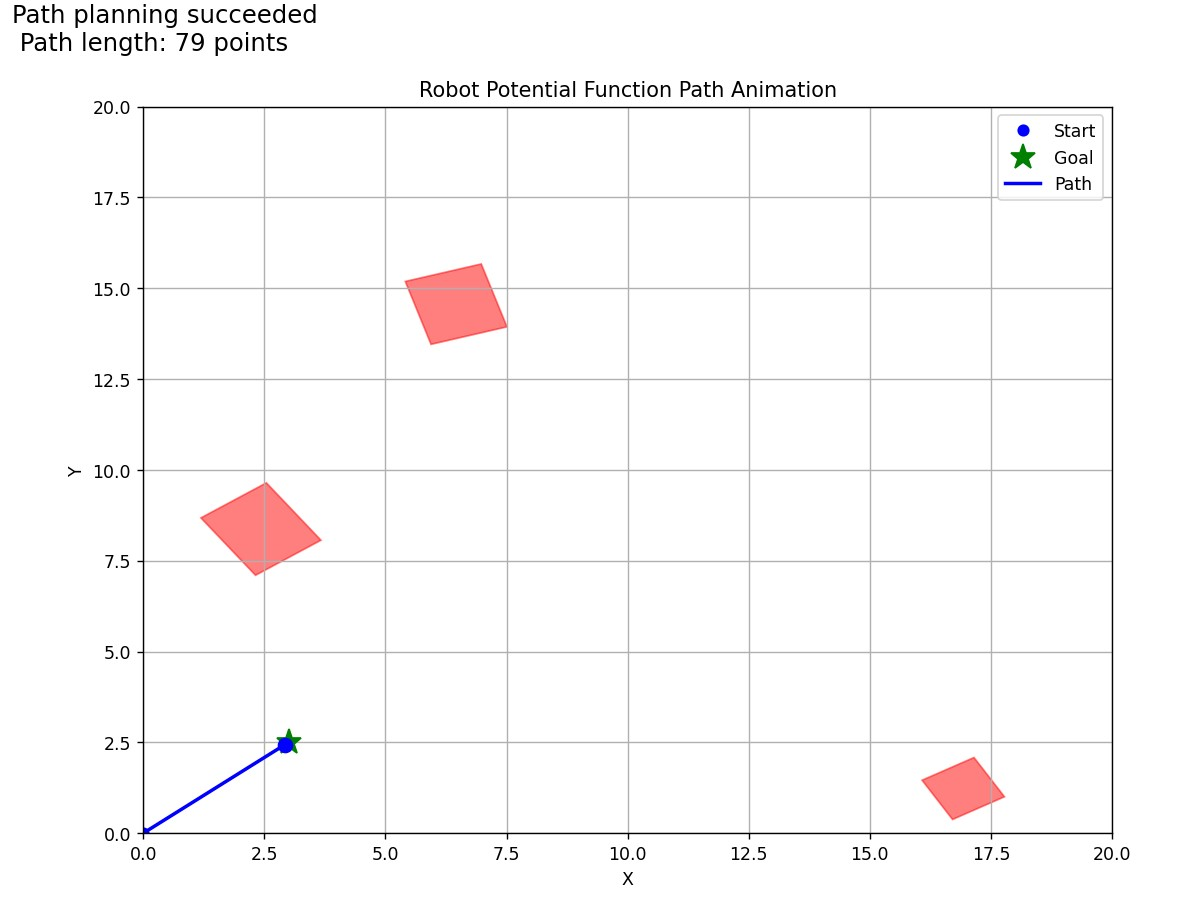
\includegraphics[width=0.5\linewidth]{latex_media/Env2PotentialTest1.jpg}
    \caption{Environment 2 Potential Test 1}
\end{figure}

\begin{figure} [H]
    \centering
    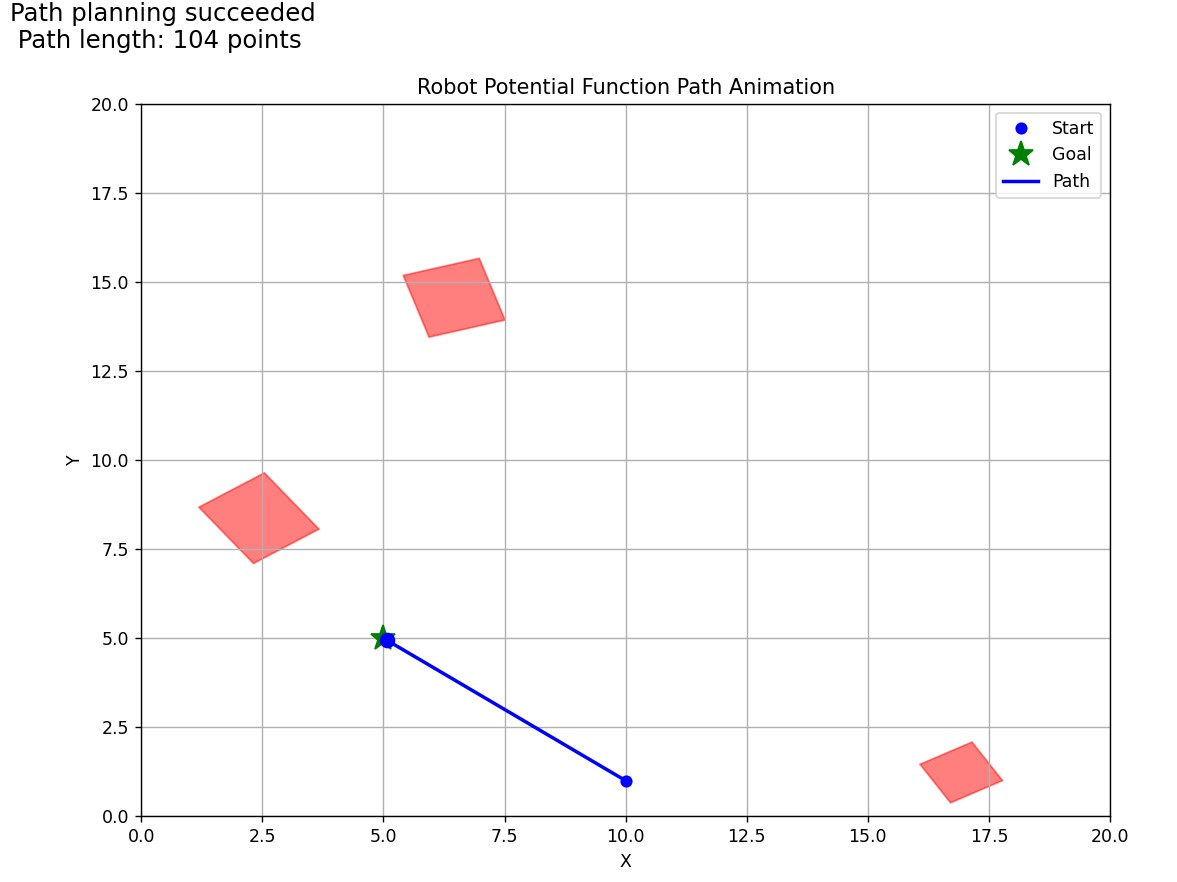
\includegraphics[width=0.5\linewidth]{latex_media/Env2PotentialTest2.jpg}
    \caption{Environment 2 Potential Test 2}
\end{figure}

\begin{figure} [H]
    \centering
    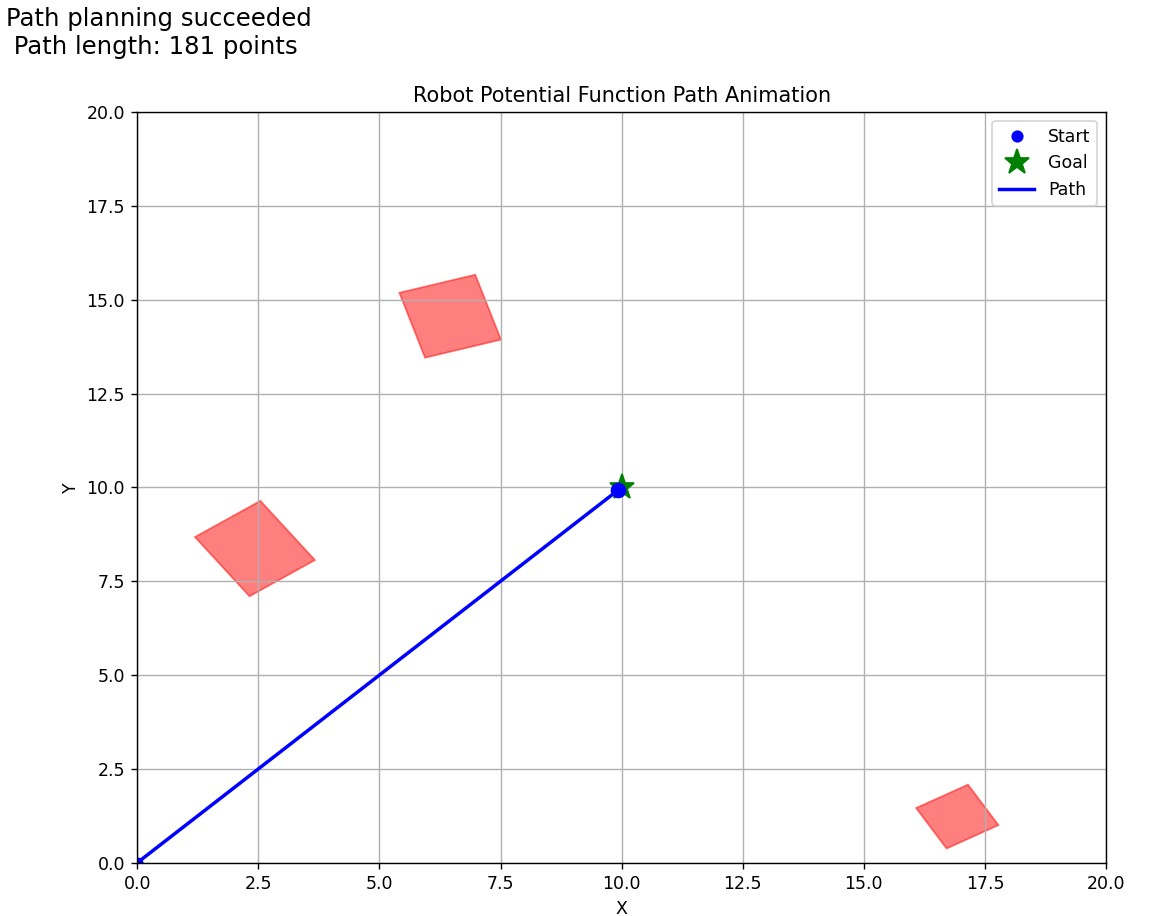
\includegraphics[width=0.5\linewidth]{latex_media/Env2PotentialTest3.jpg}
    \caption{Environment 2 Potential Test 3}
\end{figure}

\begin{figure} [H]
    \centering
    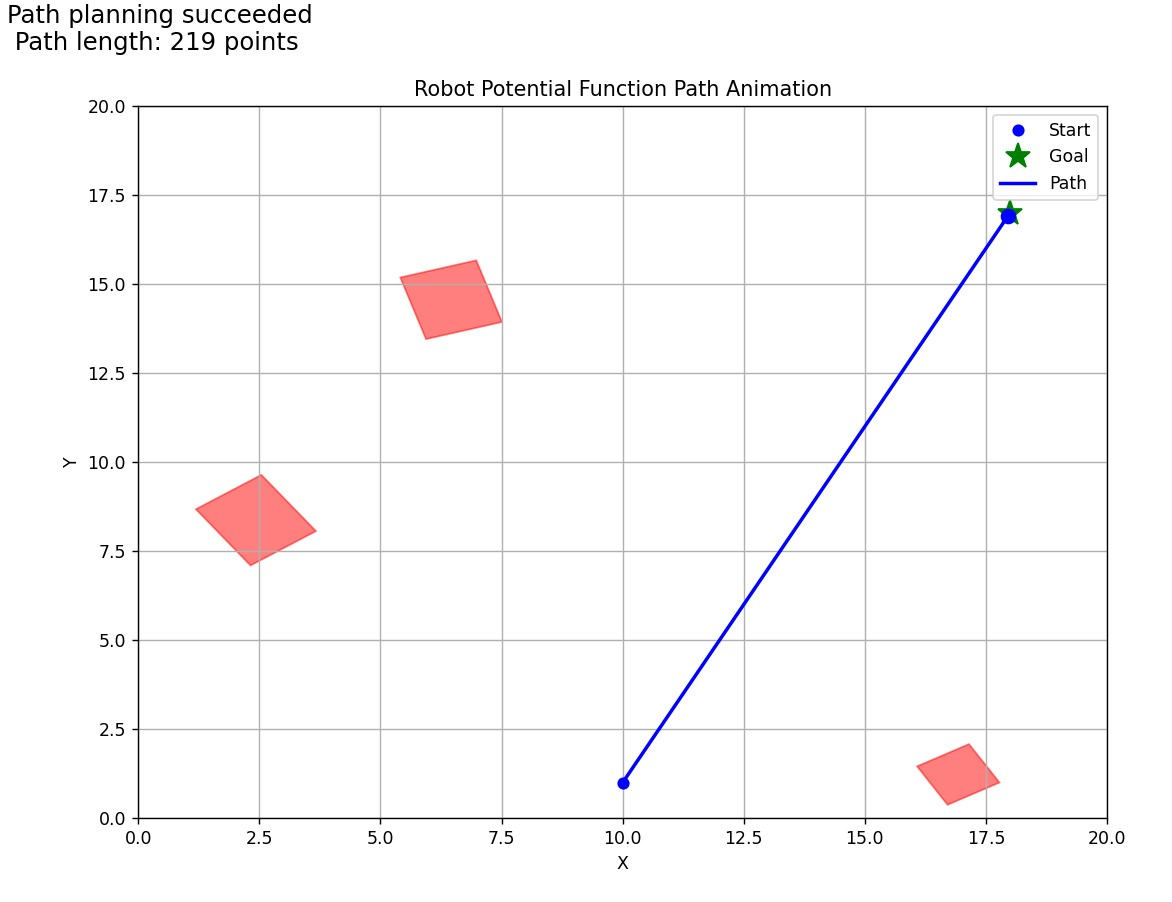
\includegraphics[width=0.5\linewidth]{latex_media/Env2PotentialTest4.jpg}
    \caption{Environment 2 Potential Test 4}
\end{figure}

\begin{figure} [H]
    \centering
    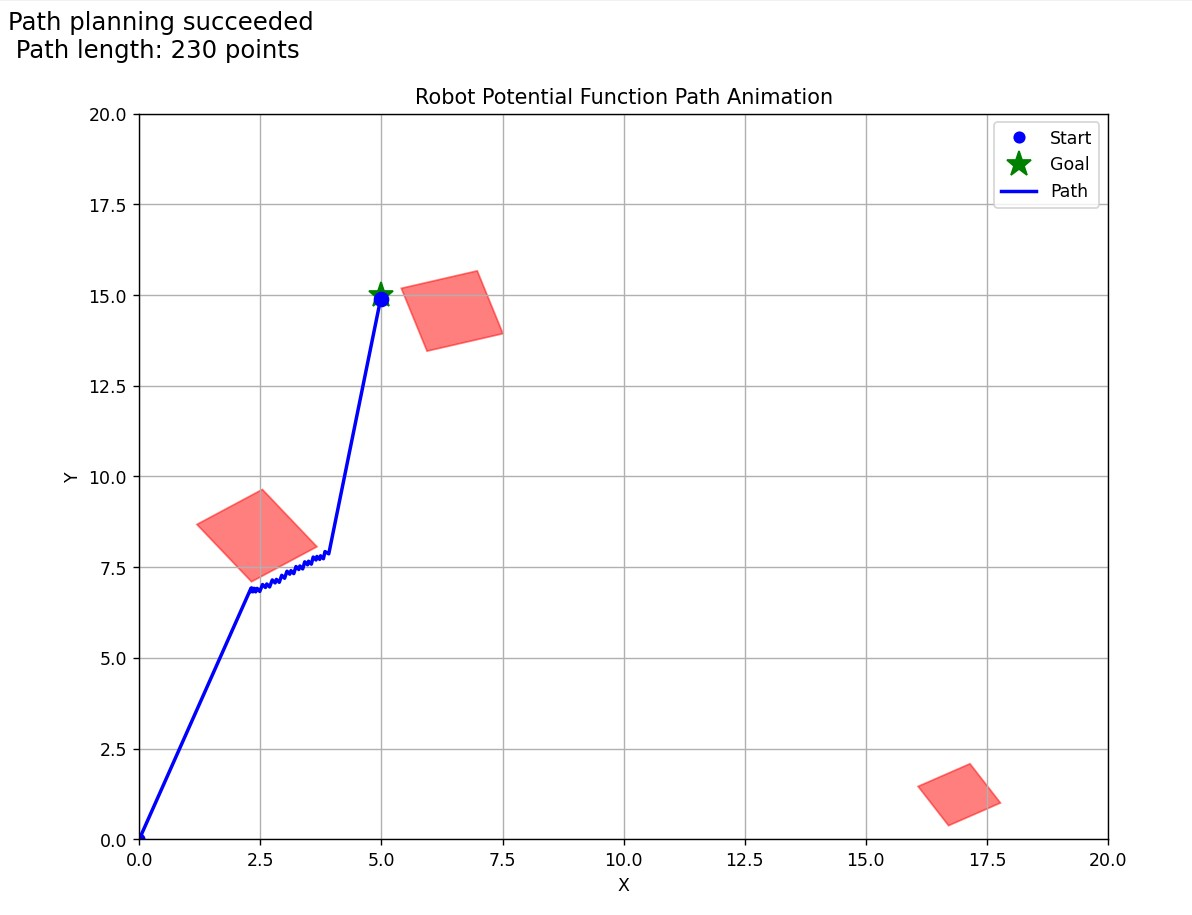
\includegraphics[width=0.5\linewidth]{latex_media/Env2PotentialTest5.jpg}
    \caption{Environment 2 Potential Test 5}
\end{figure}

\begin{figure} [H]
    \centering
    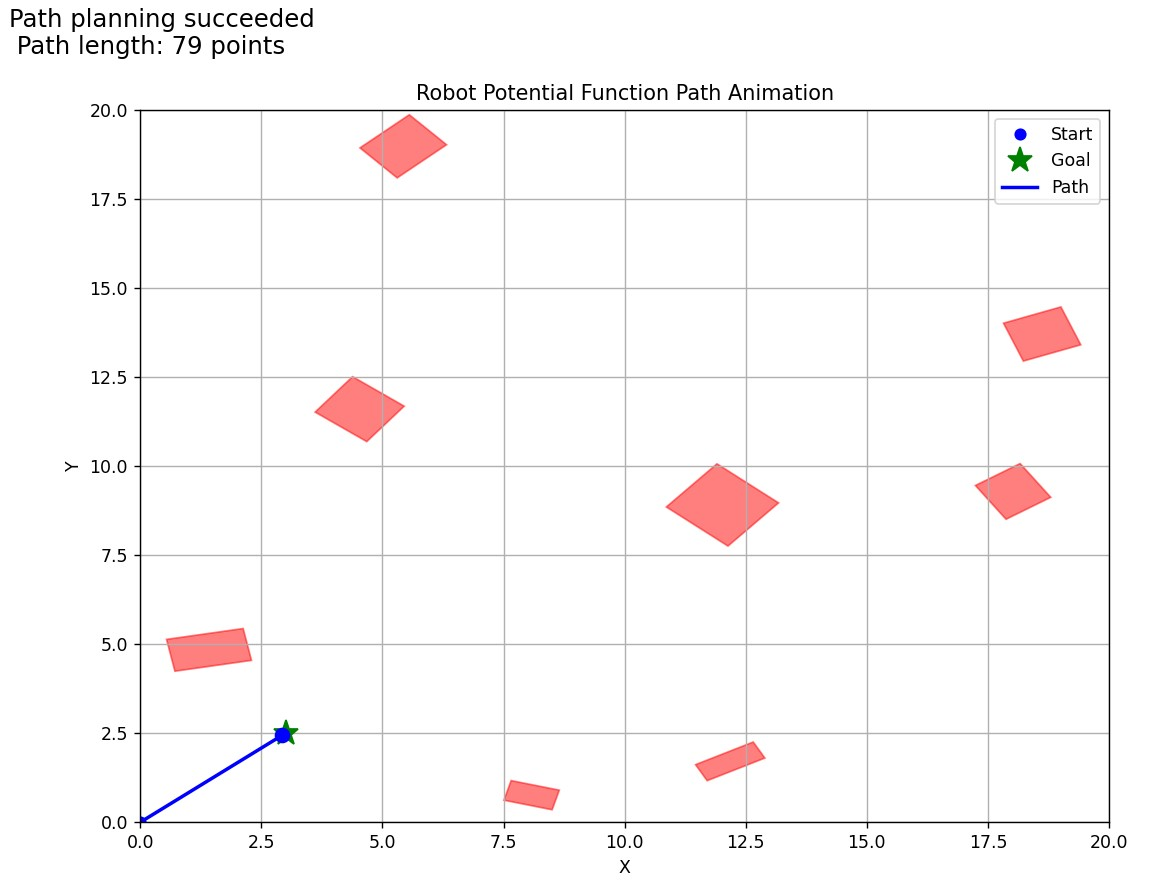
\includegraphics[width=0.5\linewidth]{latex_media/Env3PotentialTest1.jpg}
    \caption{Environment 3 Potential Test 1}
\end{figure}

\begin{figure} [H]
    \centering
    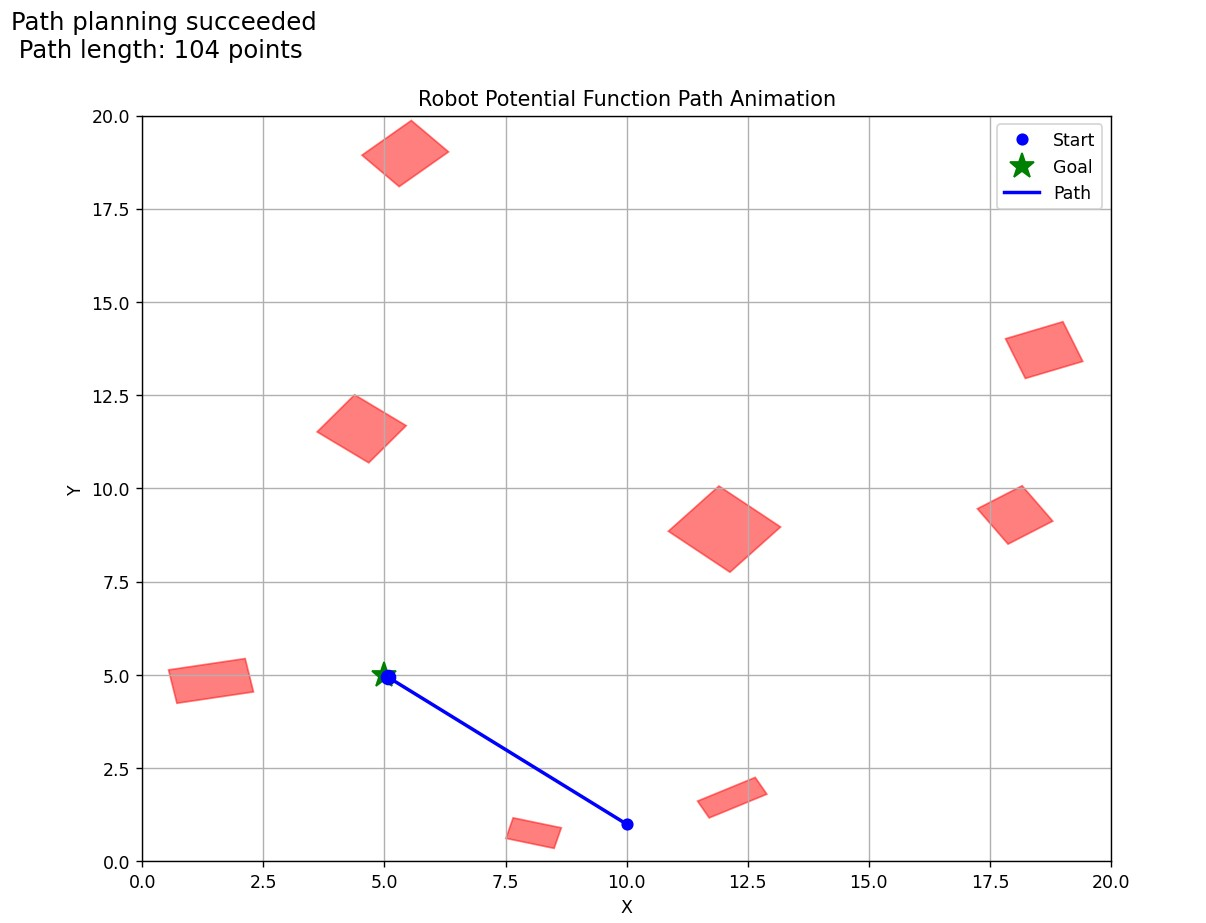
\includegraphics[width=0.5\linewidth]{latex_media/Env3PotentialTest2.jpg}
    \caption{Environment 3 Potential Test 2}
\end{figure}

\begin{figure} [H]
    \centering
    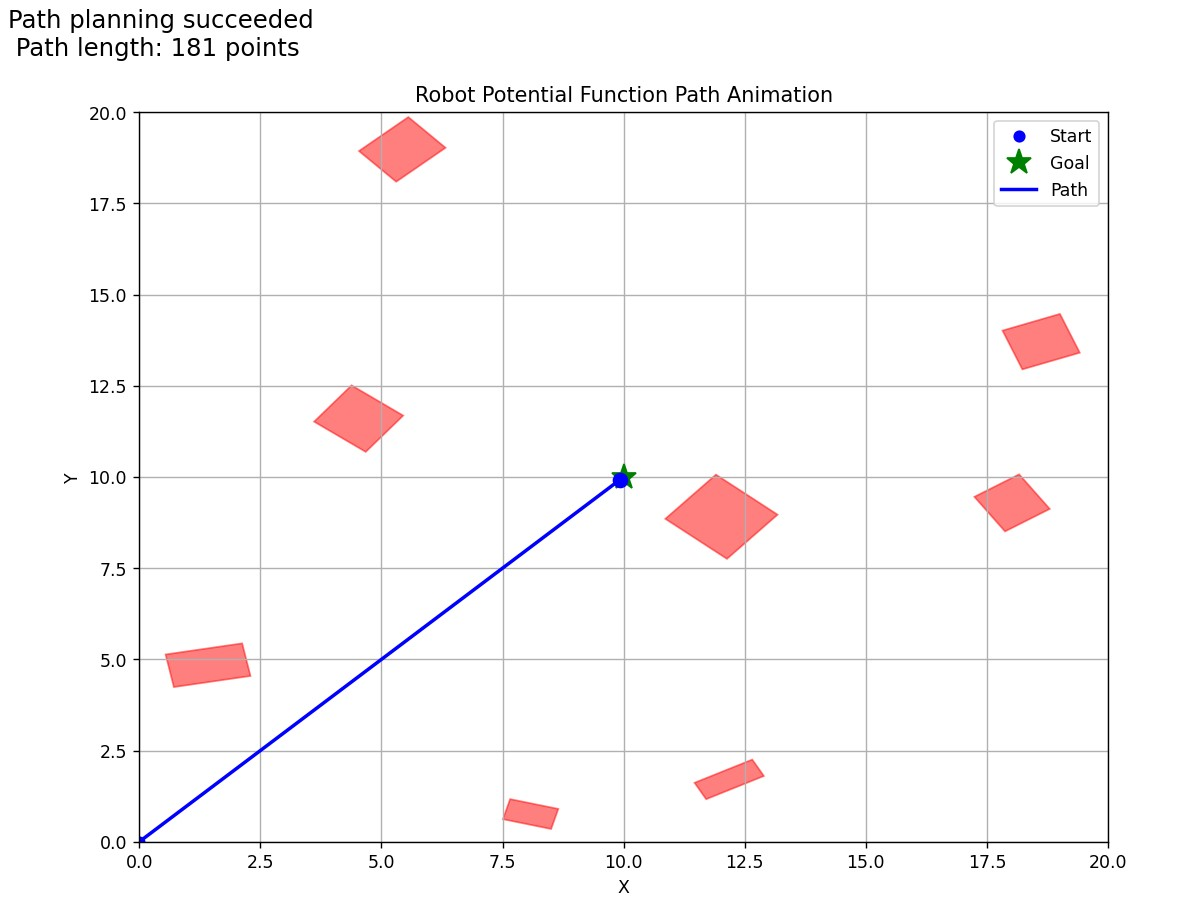
\includegraphics[width=0.5\linewidth]{latex_media/Env3PotentialTest3.jpg}
    \caption{Environment 3 Potential Test 3}
\end{figure}

\begin{figure} [H]
    \centering
    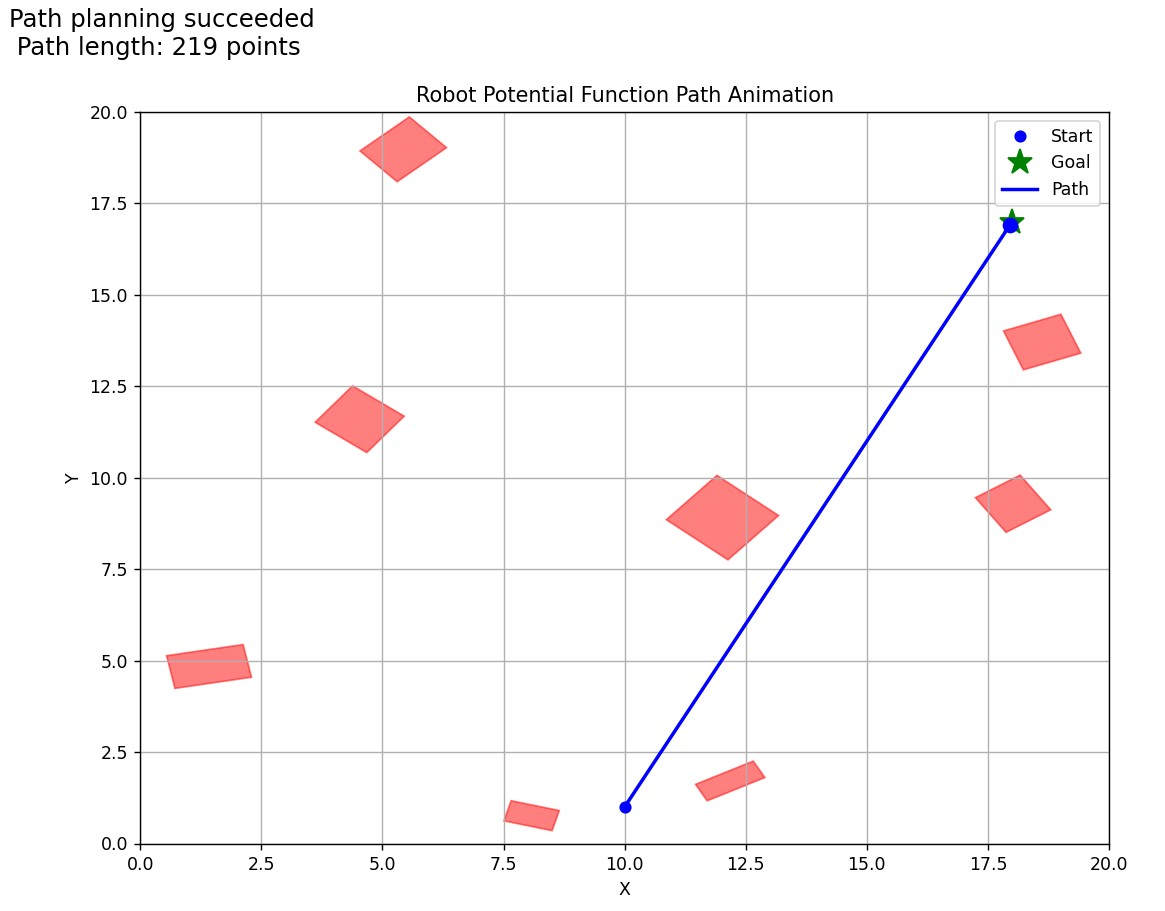
\includegraphics[width=0.5\linewidth]{latex_media/Env3PotentialTest4.jpg}
    \caption{Environment 3 Potential Test 4}
\end{figure}

\begin{figure} [H]
    \centering
    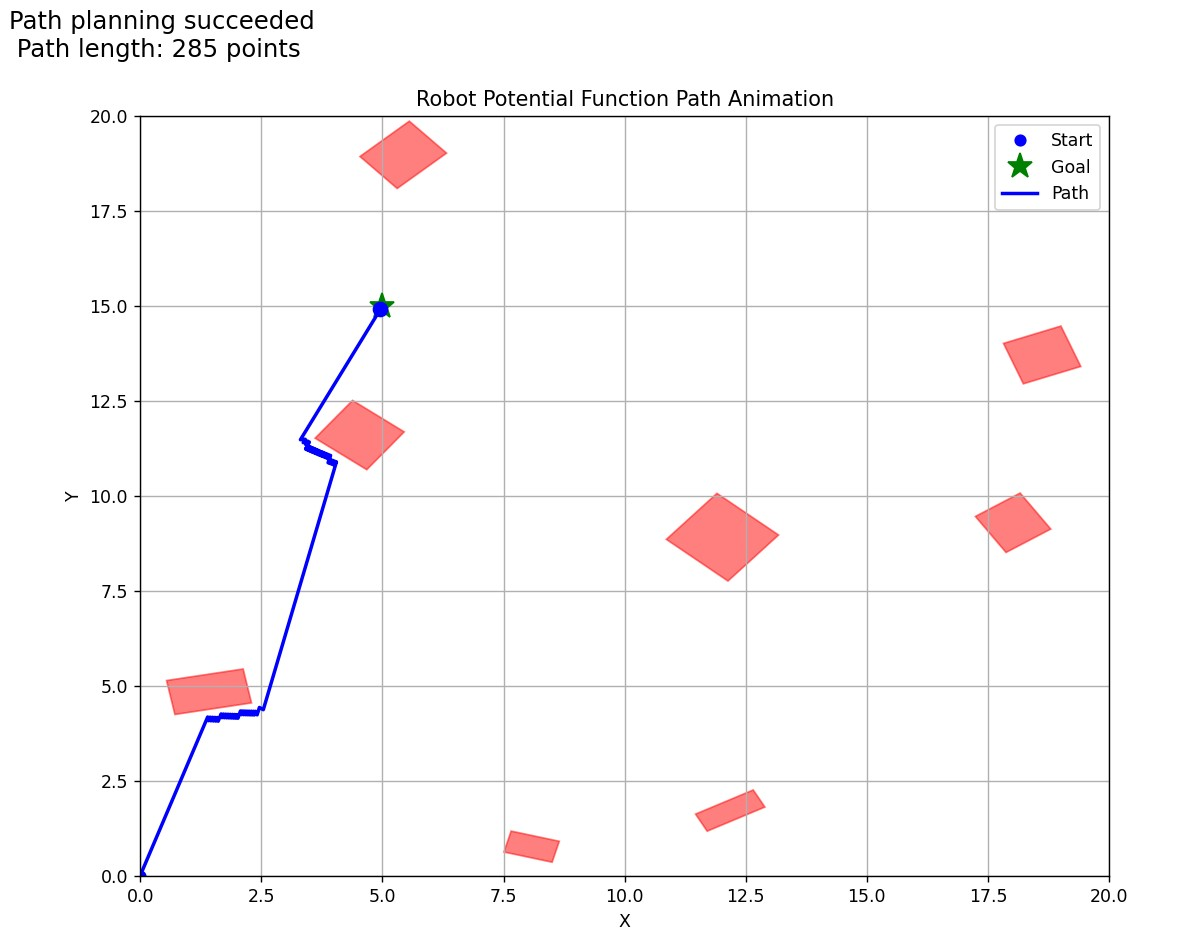
\includegraphics[width=0.5\linewidth]{latex_media/Env3PotentialTest5.jpg}
    \caption{Environment 3 Potential Test 5}
\end{figure}

\begin{figure} [H]
    \centering
    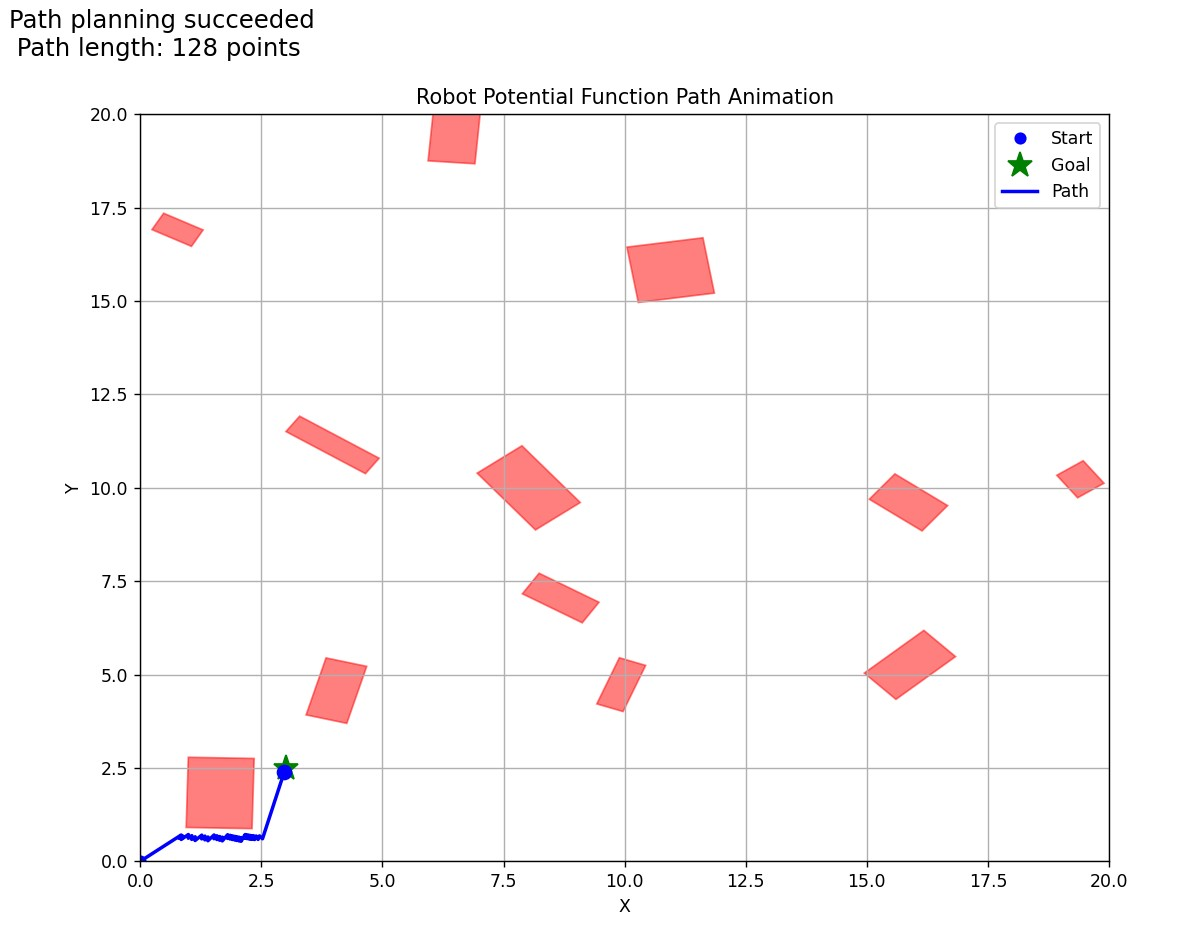
\includegraphics[width=0.5\linewidth]{latex_media/Env4PotentialTest1.jpg}
    \caption{Environment 4 Potential Test 1}
\end{figure}

\begin{figure} [H]
    \centering
    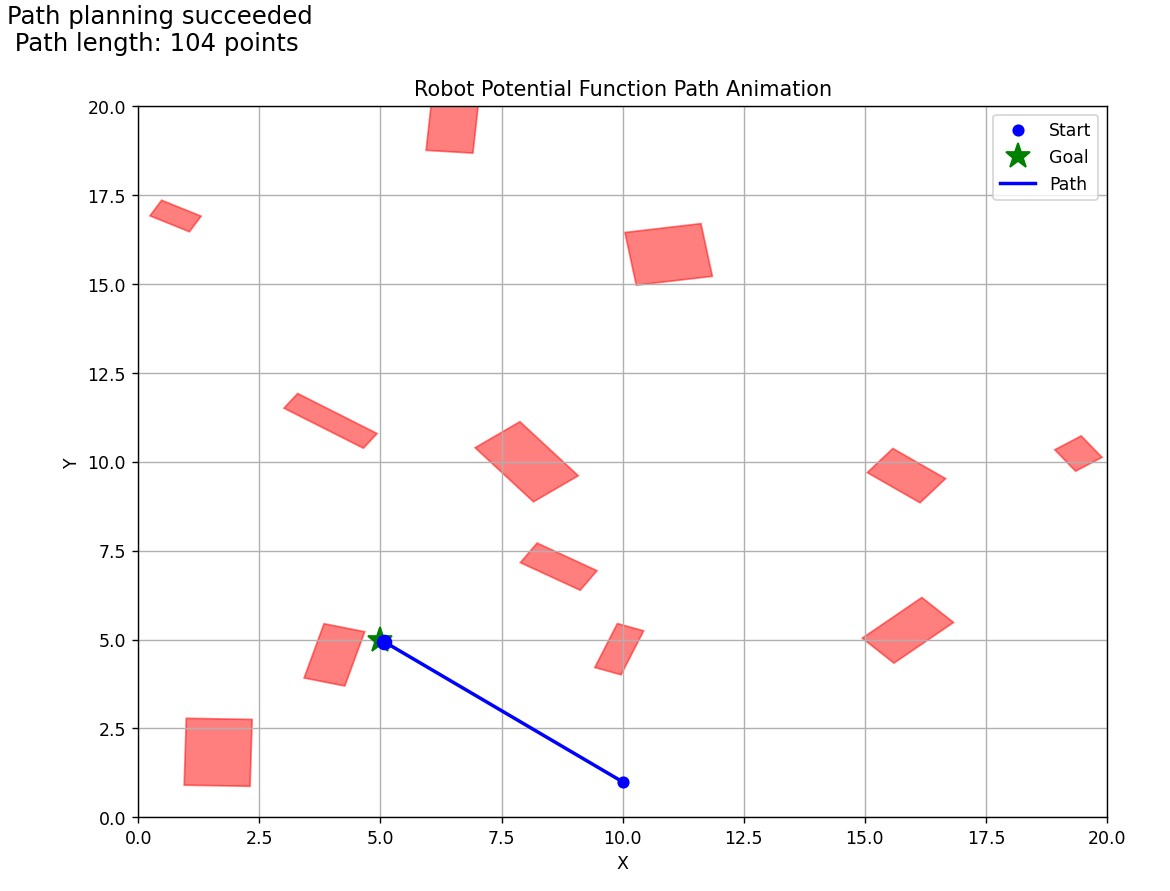
\includegraphics[width=0.5\linewidth]{latex_media/Env4PotentialTest2.jpg}
    \caption{Environment 4 Potential Test 2}
\end{figure}

\begin{figure} [H]
    \centering
    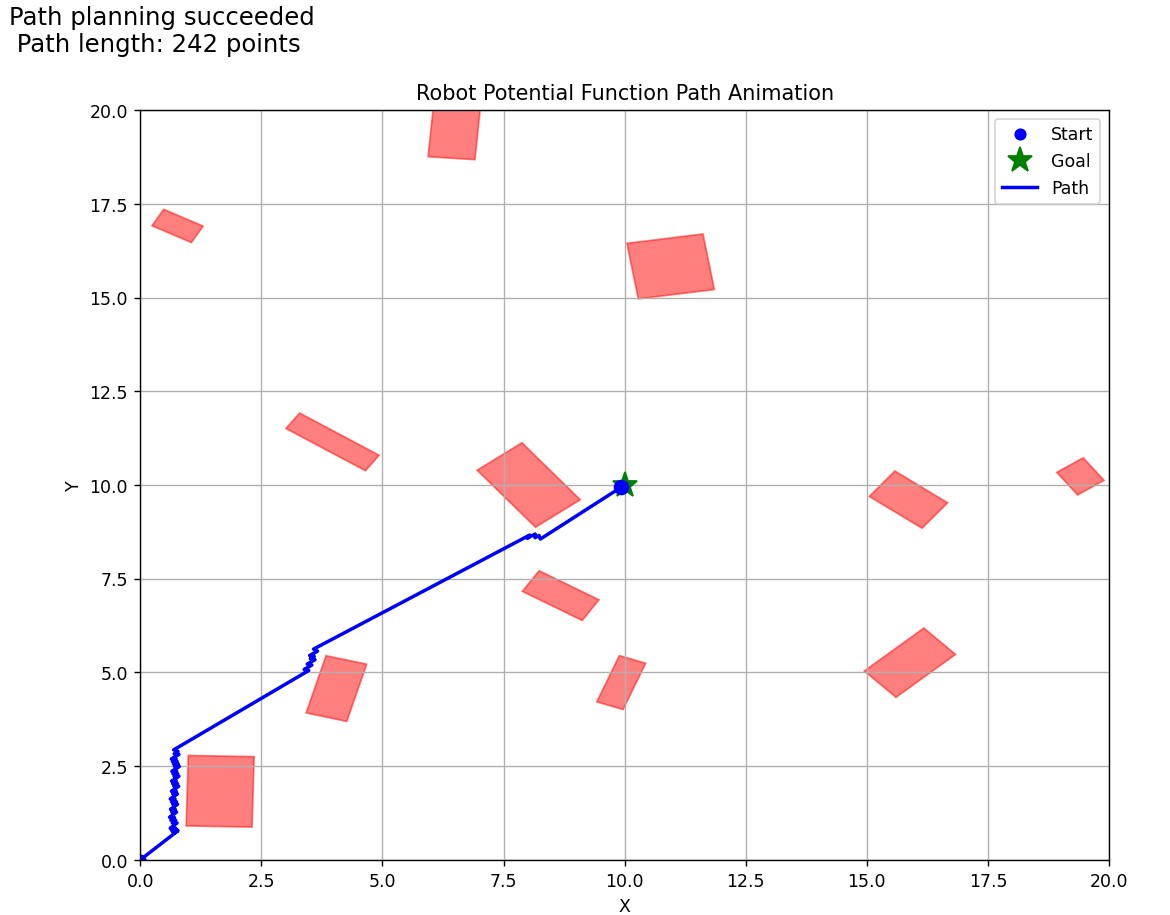
\includegraphics[width=0.5\linewidth]{latex_media/Env4PotentialTest3.jpg}
    \caption{Environment 4 Potential Test 3}
\end{figure}

\begin{figure} [H]
    \centering
    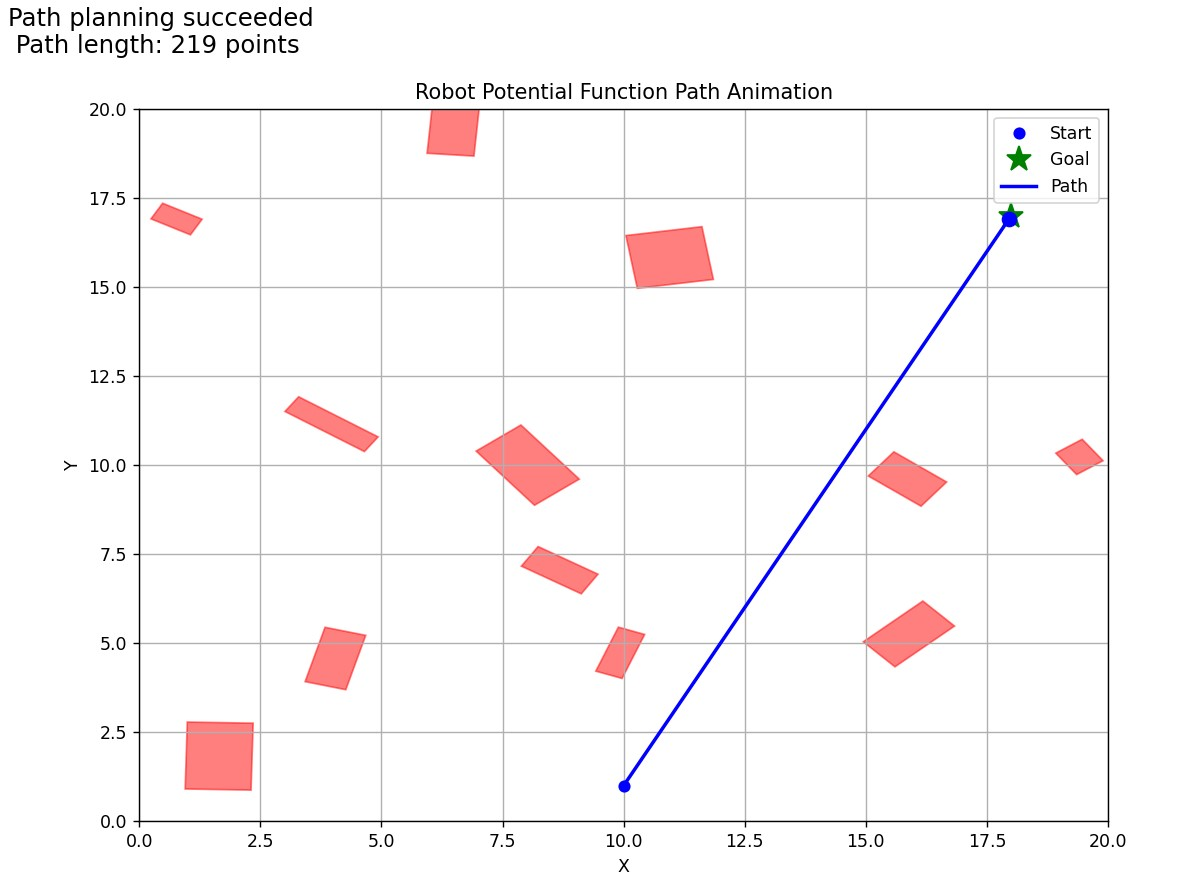
\includegraphics[width=0.5\linewidth]{latex_media/Env4PotentialTest4.jpg}
    \caption{Environment 4 Potential Test 4}
\end{figure}

\begin{figure} [H]
    \centering
    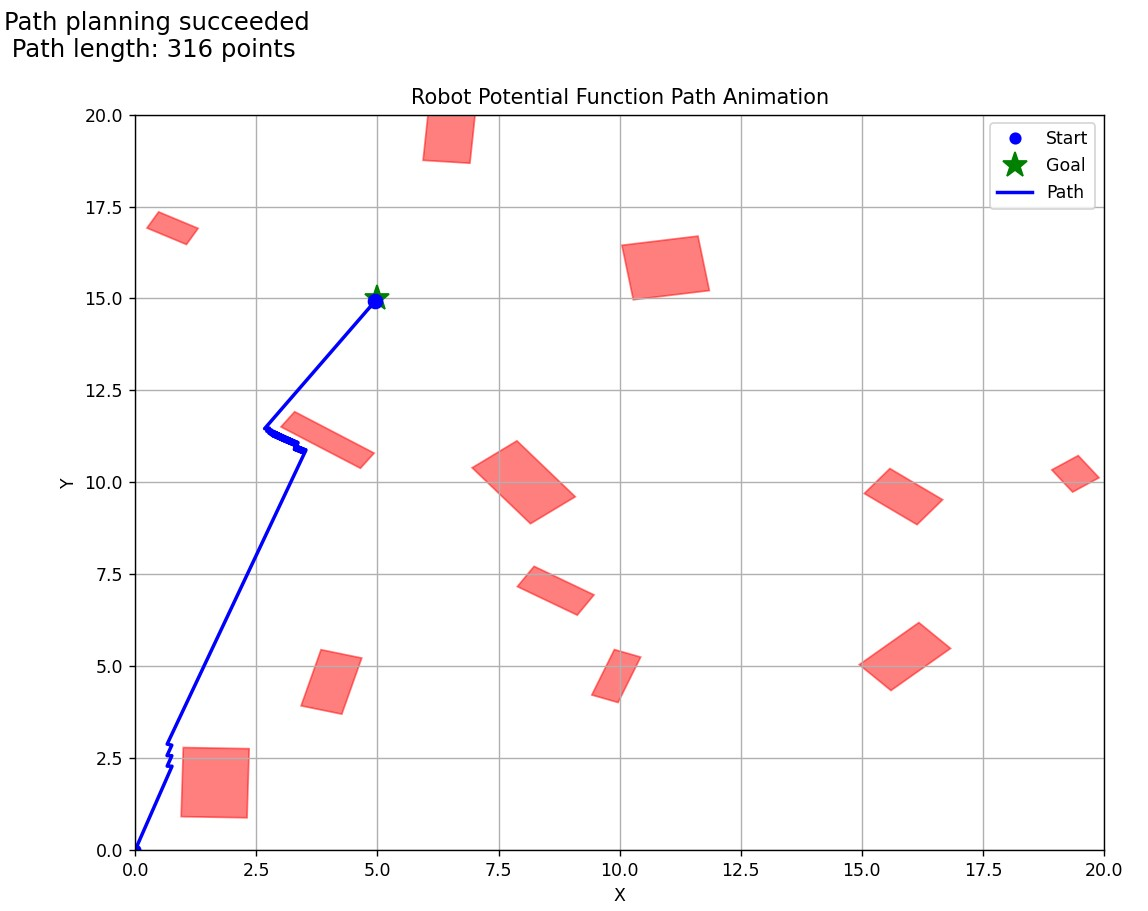
\includegraphics[width=0.5\linewidth]{latex_media/Env4PotentialTest5.jpg}
    \caption{Environment 4 Potential Test 5}
\end{figure}

\begin{figure} [H]
    \centering
    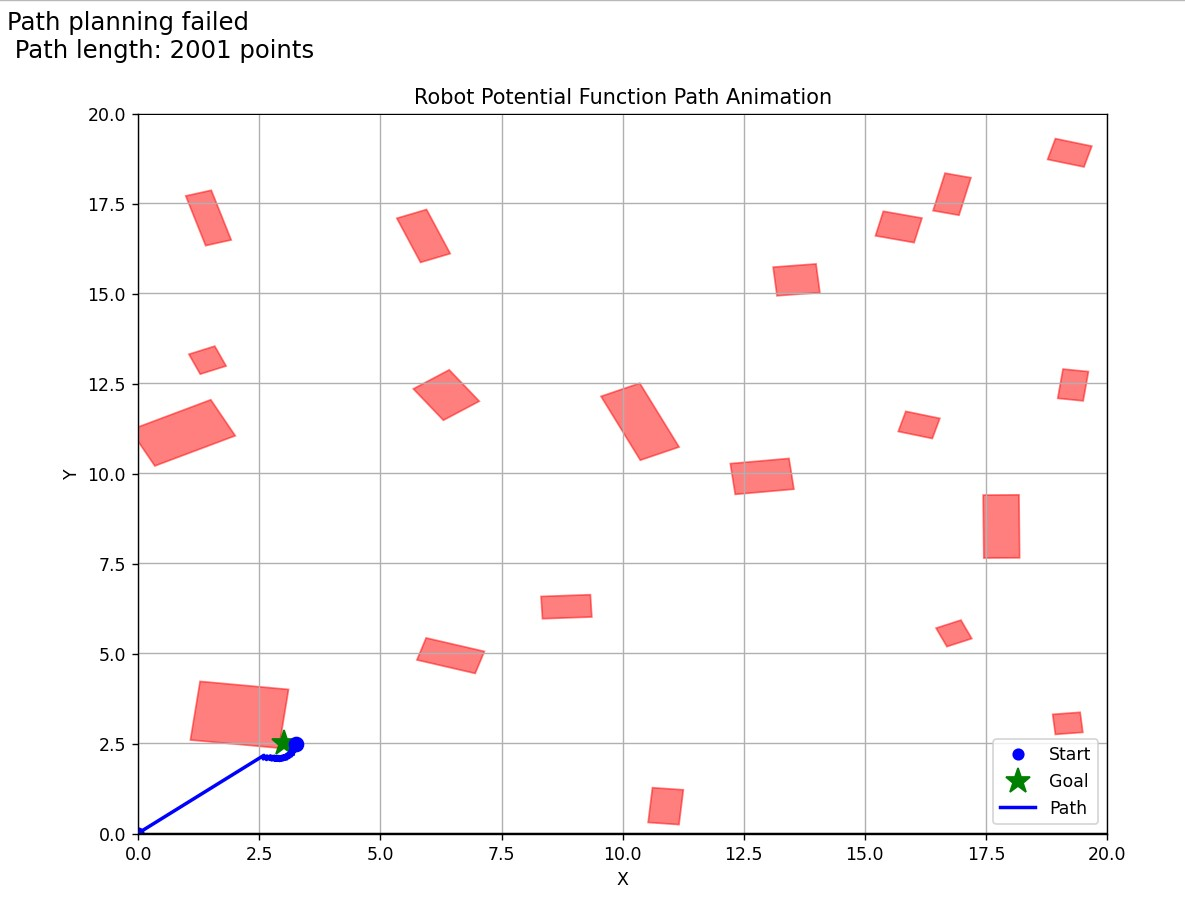
\includegraphics[width=0.5\linewidth]{latex_media/Env5PotentialTest1.jpg}
    \caption{Environment 5 Potential Test 1 (Fail)}
\end{figure}

\begin{figure} [H]
    \centering
    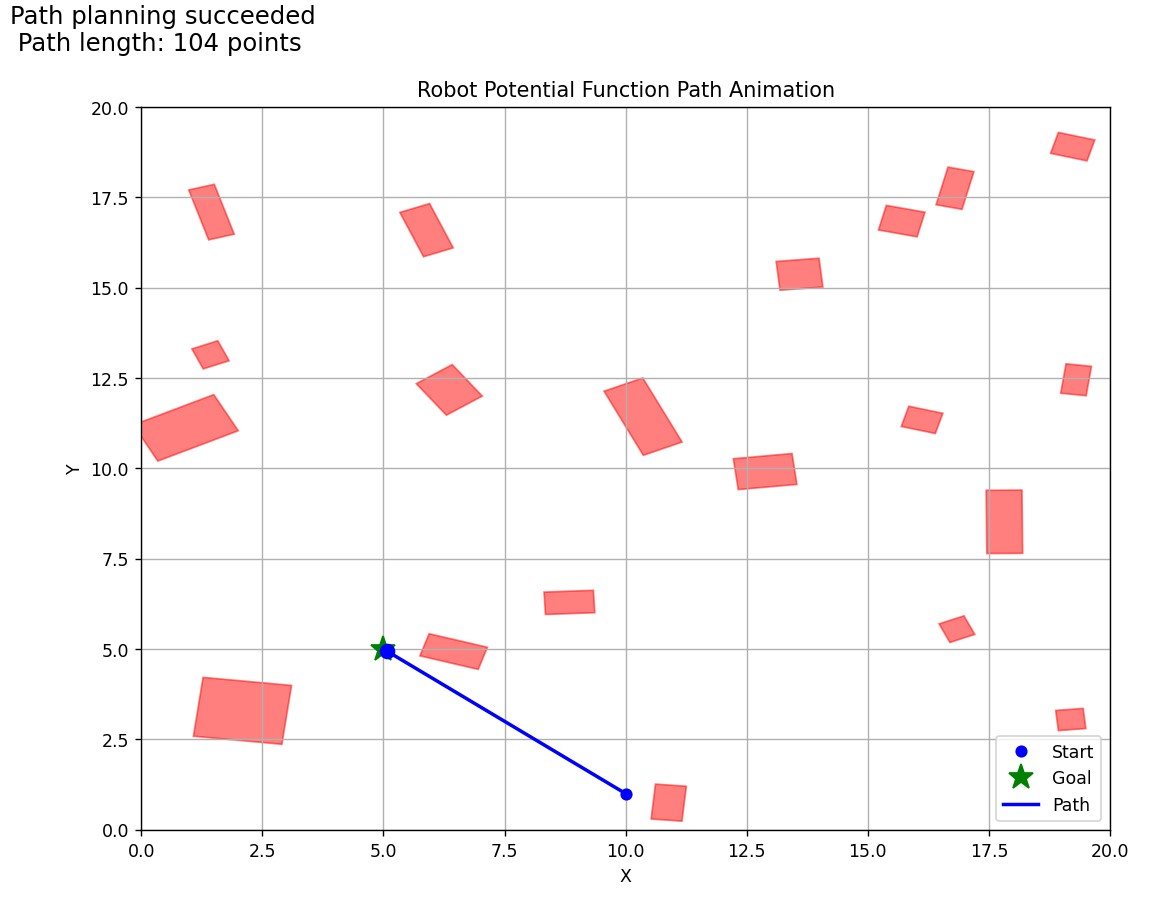
\includegraphics[width=0.5\linewidth]{latex_media/Env5PotentialTest2.jpg}
    \caption{Environment 5 Potential Test 2}
\end{figure}

\begin{figure} [H]
    \centering
    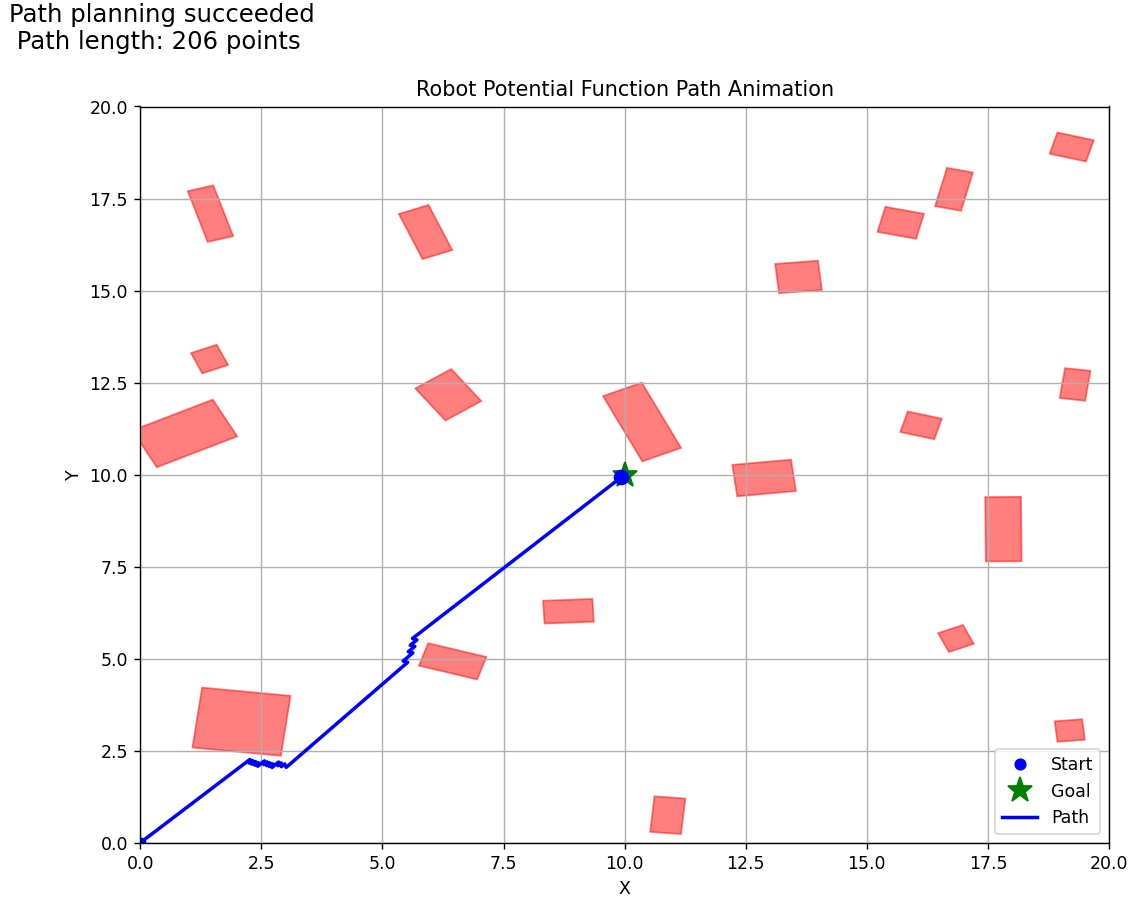
\includegraphics[width=0.5\linewidth]{latex_media/Env5PotentialTest3.jpg}
    \caption{Environment 5 Potential Test 3}
\end{figure}

\begin{figure} [H]
    \centering
    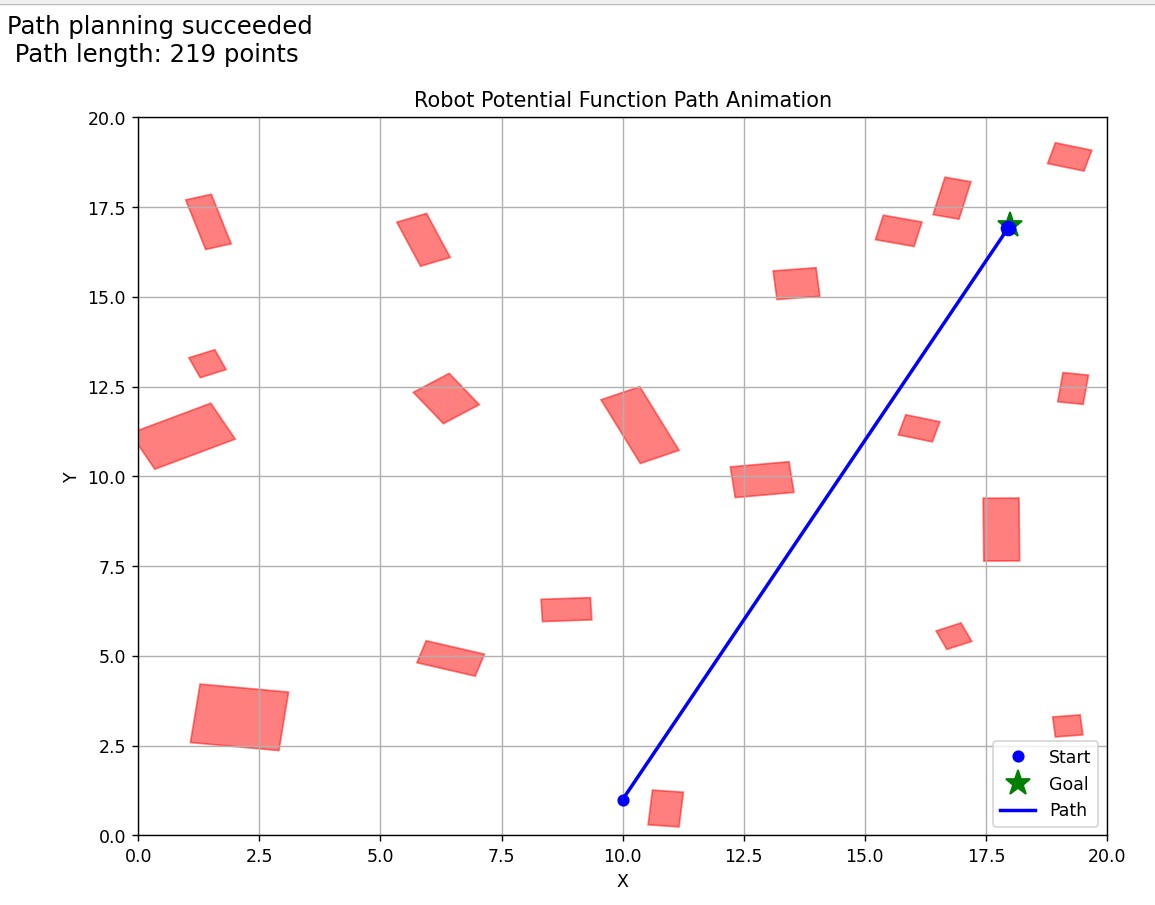
\includegraphics[width=0.5\linewidth]{latex_media/Env5PotentialTest4.jpg}
    \caption{Environment 5 Potential Test 4}
\end{figure}

\begin{figure} [H]
    \centering
    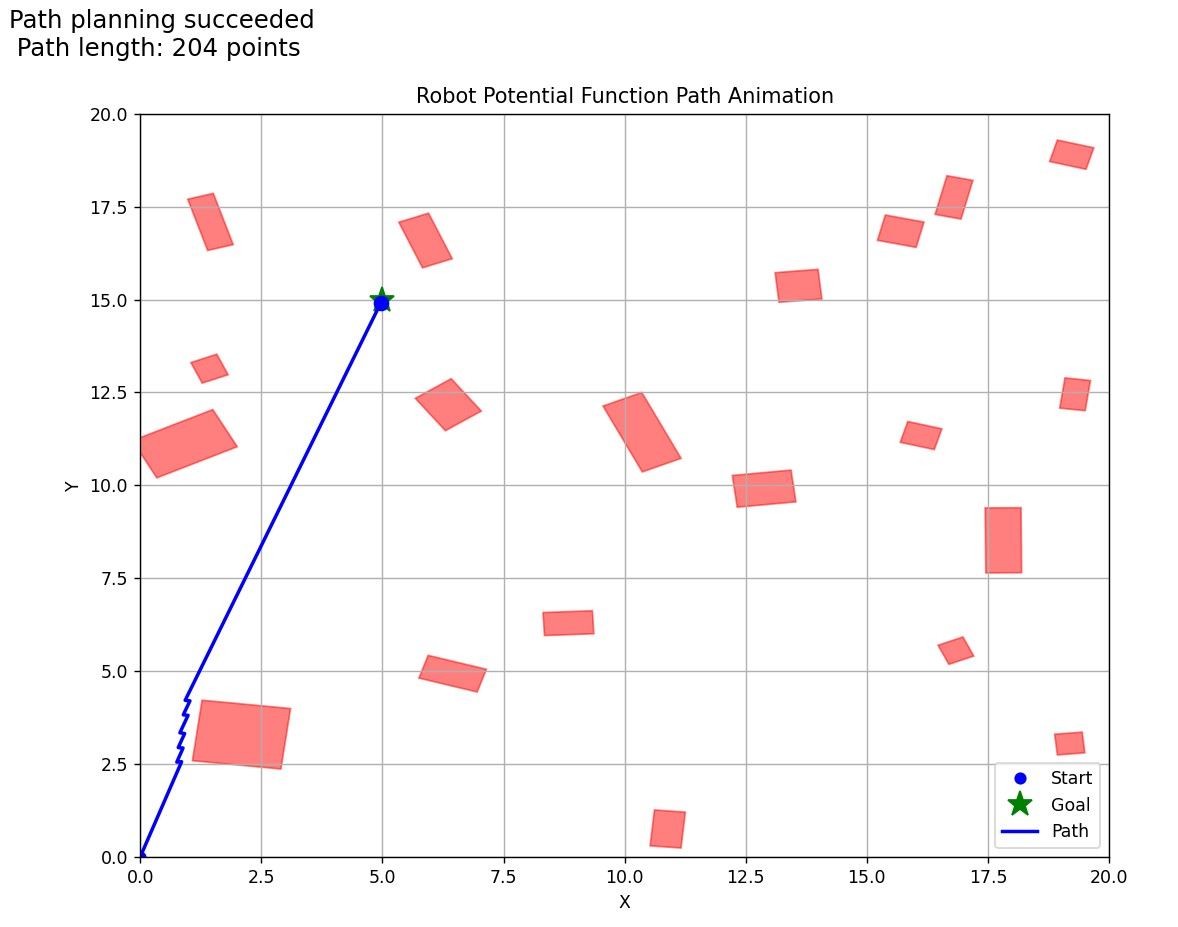
\includegraphics[width=0.5\linewidth]{latex_media/Env5PotentialTest5.jpg}
    \caption{Environment 5 Potential Test 5}
\end{figure}

\section{GTSAM: Factor Graphs}
Given the sample code from the assignment details file, adjusting the Python script to fit a third-order polynomial involves changing a few things. For instance, we adapted the "true" function definition to fit the polynomial $a\cdot x^3 + b\cdot x^2 + c\cdot x + d$. Similarly, we redefined each variable in the \texttt{error\_func} function to conform to the new polynomial, including changing the Jacobians.

\begin{figure} [H]
    \centering
    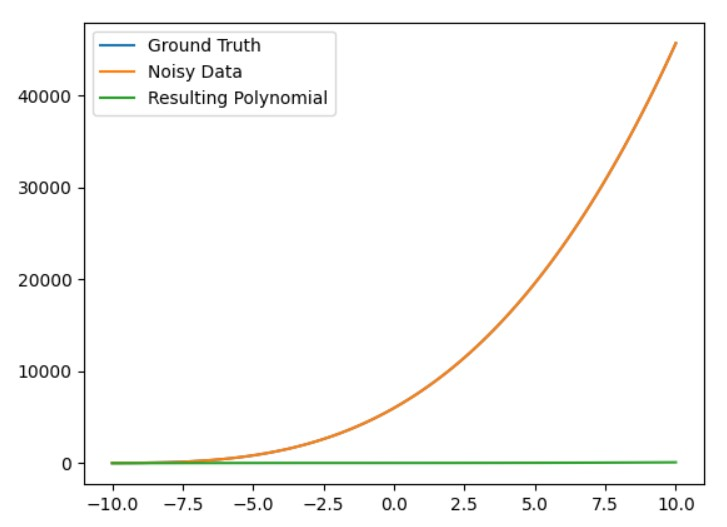
\includegraphics[width=0.8\linewidth]{latex_media/polynomial_factor_graph_sigma1.jpg}
    \caption{Polynomial-fitting factor graph with $\sigma = 1$}
\end{figure}

\begin{figure} [H]
    \centering
    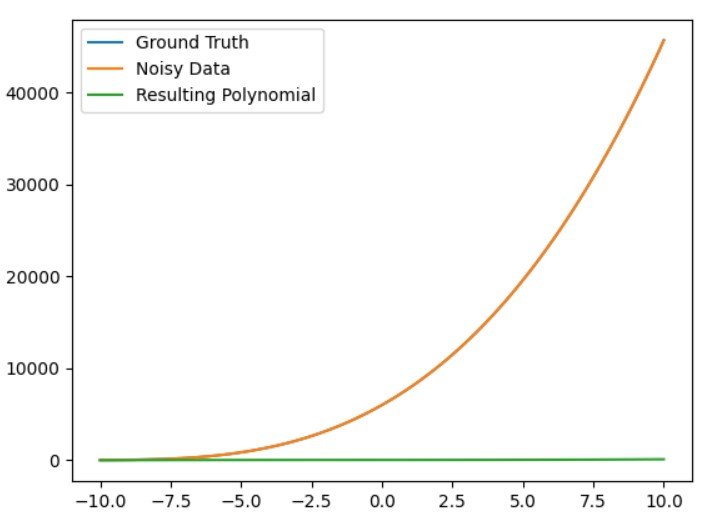
\includegraphics[width=0.8\linewidth]{latex_media/polynomial_factor_graph_sigma5.jpg}
    \caption{Polynomial-fitting factor graph with $\sigma = 5$}
\end{figure}

\begin{figure} [H]
    \centering
    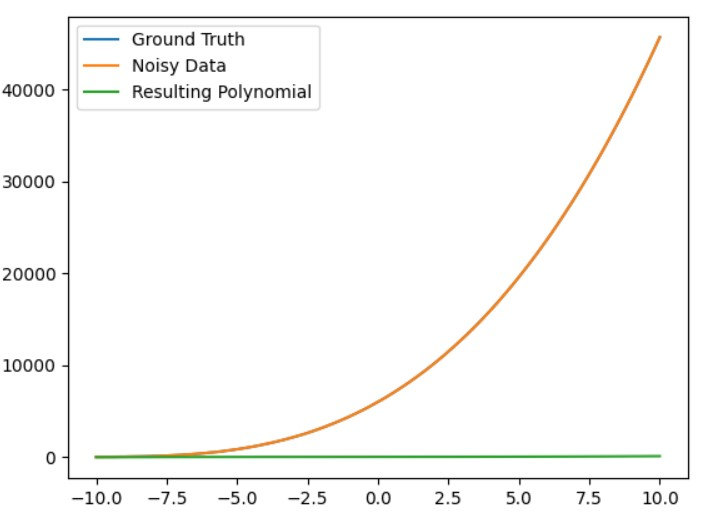
\includegraphics[width=0.8\linewidth]{latex_media/polynomial_factor_graph_sigma10.jpg}
    \caption{Polynomial-fitting factor graph with $\sigma = 10$}
\end{figure}

Note that the graphs above show the ground truth, noisy data, and the estimated polynomial, which all appear the same. Although they look similar, the values are slightly different from one another. For instance, the estimates for $a$, $b$, $c$, and $d$ for $\sigma = 1,5,10$, respectively, are \\

\noindent
a: 0.04500272879773473, b: 0.19975365635782394, c: 0.7027278716643242, d: 4.870233319918706 \newline
a: 0.04504021776744929, b: 0.19410772251519173, c: 0.9272714408832875, d: 3.2494289869859174 \newline
a: 0.04505937872219211, b: 0.19078472726022763, c: 1.0236805442589618, d: 5.775141257404677 \newline

The graphs, however, do not accurately depict these minute differences due to the scale of the y-axis, resulting in eerily similar plots.

\section{Trajectory Optimization via Factor Graphs}


\subsection{Simple Trajectory}
We continued using the GTSAM library to help create the factor graphs for the robot's trajectory optimization. Here our goal was to compute an optimal trajectory for a robot in 2D space from start to goal. We used a fixed number of time steps T with the dynamics equation, which used the next state's position based on the current position and velocity multiplied with time step. The jacobians were calculated for error with these variables for the factor graph to optimize. The factor graph started with the priors being added, which were the start and goal positions, to directly constrain the first and last positions of the trajectory. Then the dynamics factors were added to enforce the equation by calculating the trajectory error and adding it as a factor to link the consecutive time step positions. We additionally added smoothness factors for velocity to make sure the optimizer was able to have sufficient constraints to refine the error so the velocity would remain consistent across time steps. For the initial guess of positions, we just used linear interpolation between the start and goal points, and for velocity, we used constant values based on total distance over time. These were not needed since we also tested the initial guesses on just 0,0, and we got the same results, but this would just make the optimizer have to do less work in that sense. We use the same Levenberg-Marquardt optimizer for all factor graph optimizations to minimize total error across all factors, in this case, the position and velocities at the time steps. In our factor graph design, you can see the variables are the positions and velocities, and the factors are the priors and dynamics constraints. You can see from the visuals of the trajectory the optimizer is a straight line since the constraints are well-defined. The more time steps, the more you'll have a cluster of points.

\begin{figure} [H]
    \centering
    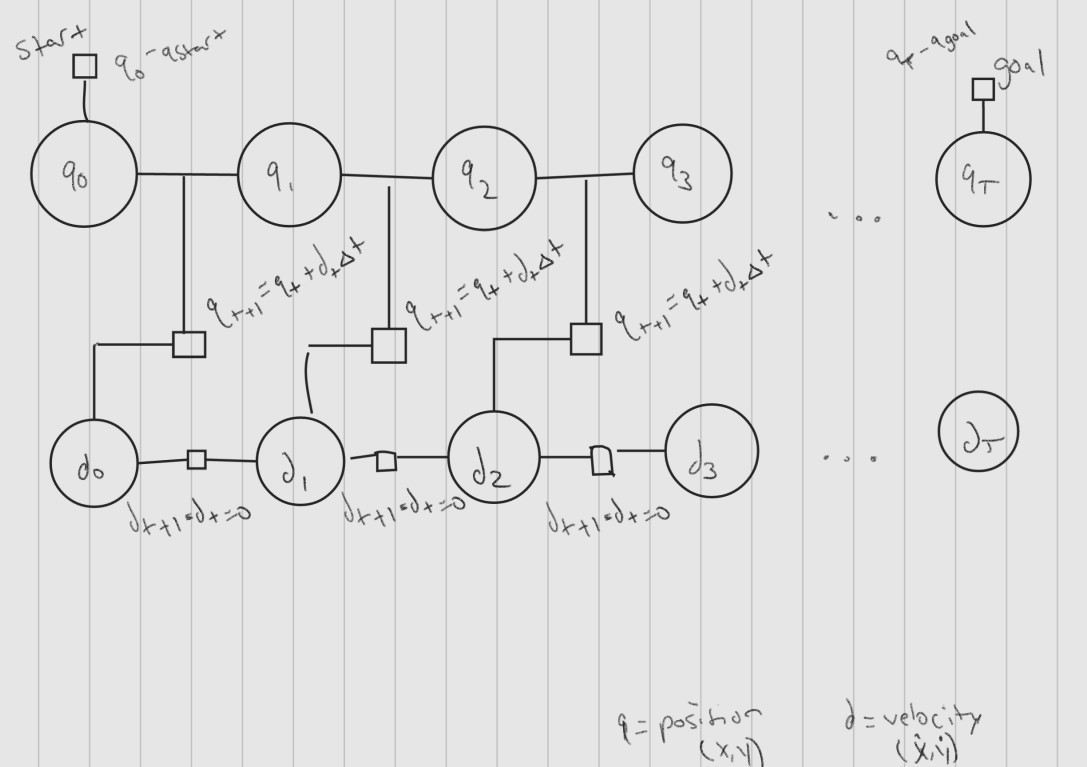
\includegraphics[width=0.5\linewidth]{latex_media/fg_traj_opt_factorGraph.jpg}
    \caption{3.1 Factor Graph}
    \label{fig:enter-label}
\end{figure}

\begin{figure} [H]
    \centering
    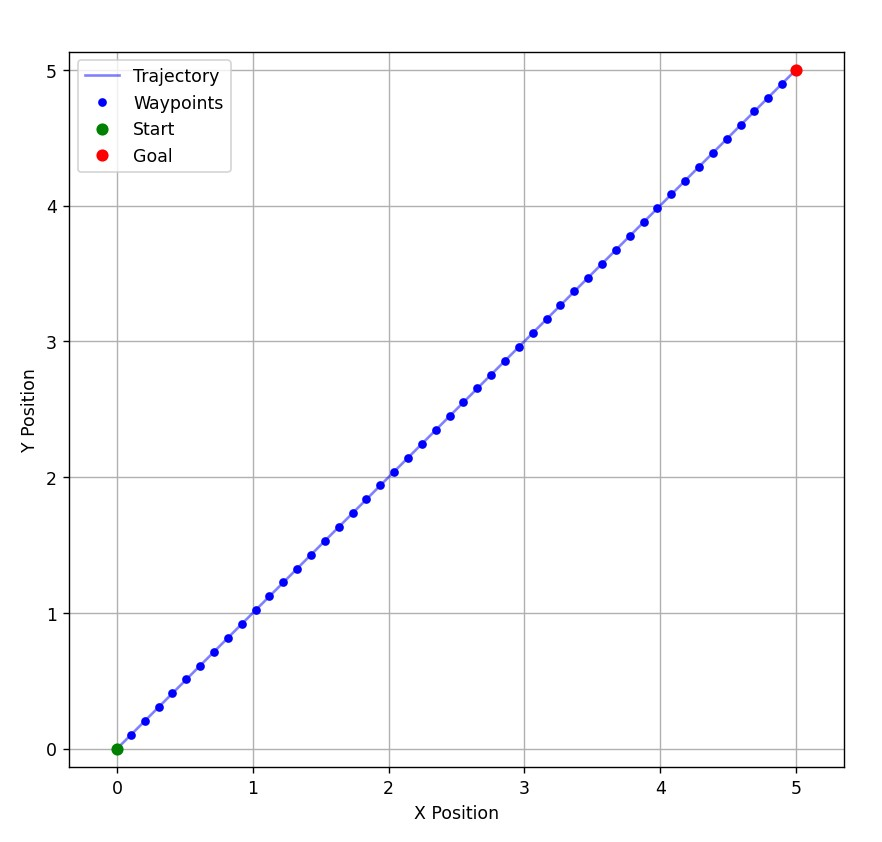
\includegraphics[width=0.5\linewidth]{latex_media/fg_traj_opt_1.jpg}
    \caption{python fg\_traj\_opt.py --start 0 0 --goal 5 5 --T 50}
    
\end{figure}

\begin{figure} [H]
    \centering
    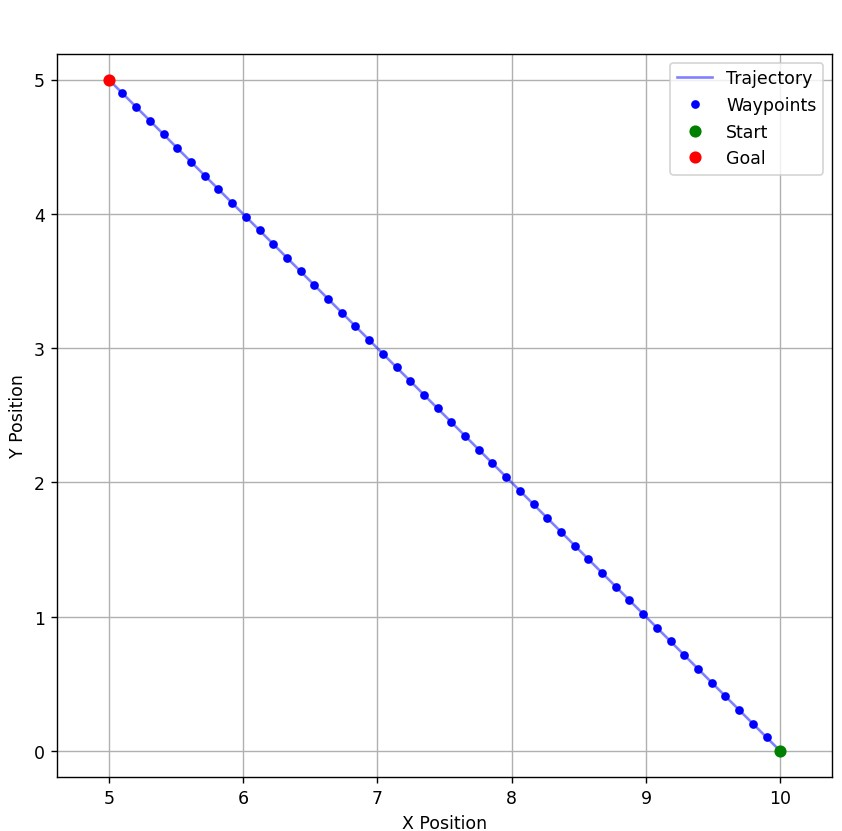
\includegraphics[width=0.5\linewidth]{latex_media/fg_traj_opt_2.jpg}
    \caption{python fg\_traj\_opt.py --start 10 0 --goal 5 5 --T 50}
    
\end{figure}

\begin{figure} [H]
    \centering
    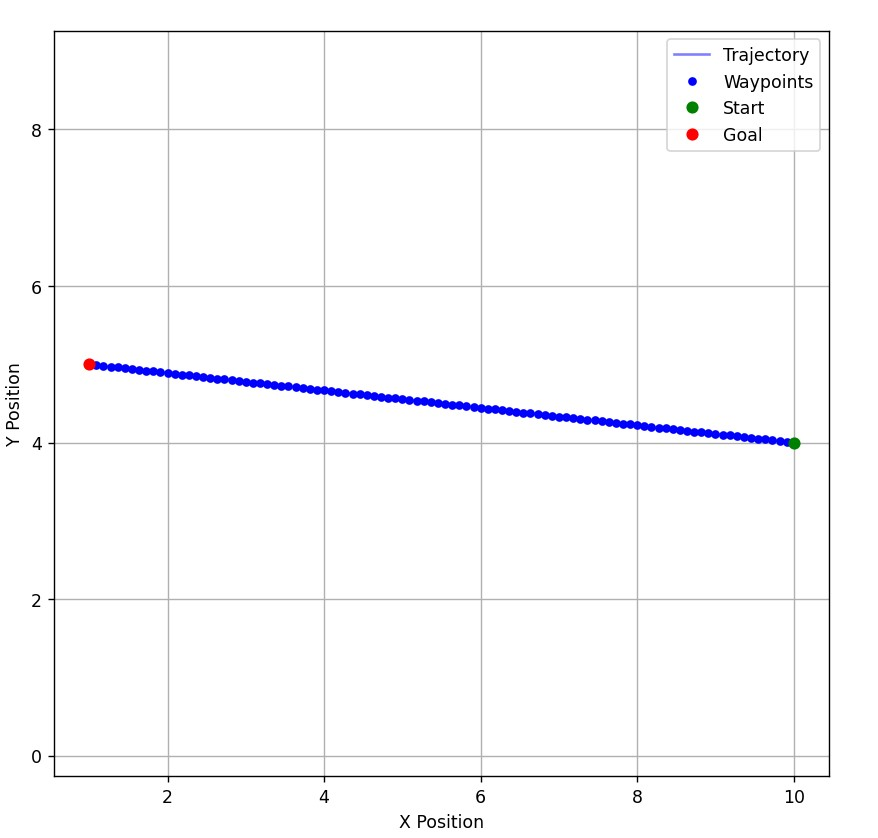
\includegraphics[width=0.5\linewidth]{latex_media/fg_traj_opt_3.jpg}
    \caption{python fg\_traj\_opt.py --start 10 4 --goal 1 5 --T 100}
    
\end{figure}



\subsection{Extra Constraints}
This factor graph optimization is relatively the same as the last one, except it has the addition of intermediate priors. These constrain the positions at specific time steps ($\frac{T}{3}$) and ($\frac{2T}{3}$) to whatever the user defines when running the program. Basically, you can see in the visuals that the trajectory goes around or into the specific points defined at the intermediate priors. You can see below our factor graph has the added intermediate priors. The visualization is the same as the last part, except we can see how the trajectory changes based on the states inputted. We also see that the more time steps we have, the more accurate the trajectory becomes. 

\begin{figure} [H]
    \centering
    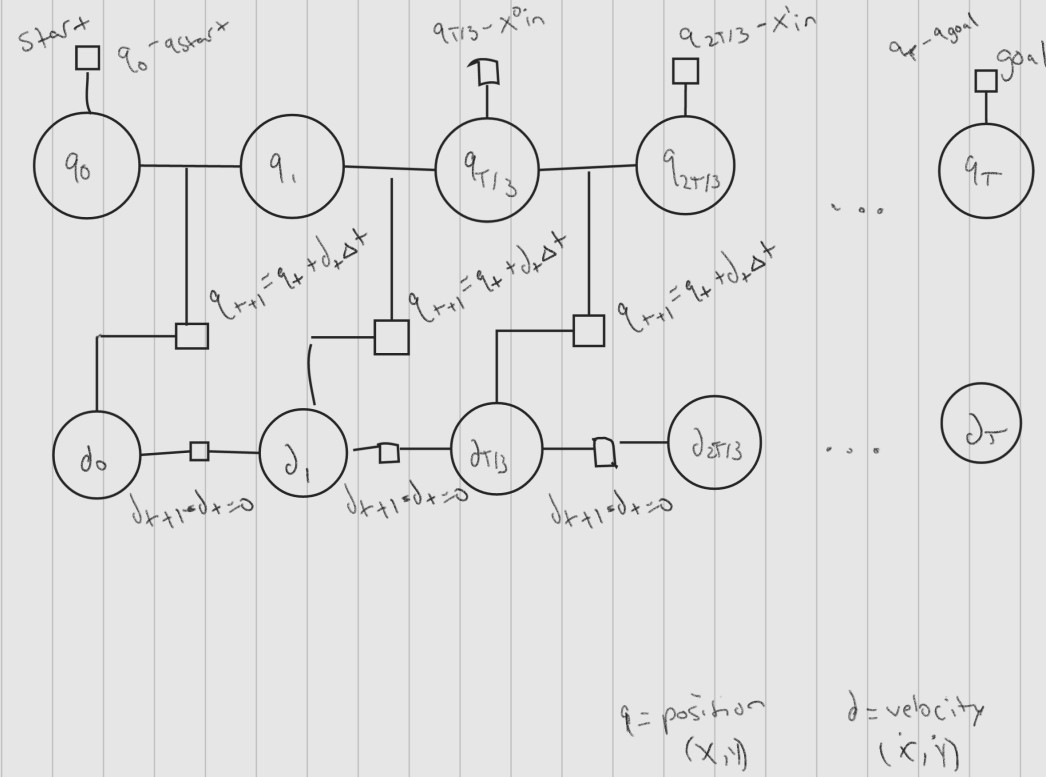
\includegraphics[width=0.5\linewidth]{latex_media/fg_traj_opt_constrained_factorGraph.jpg}
    \caption{3.2 Factor Graph}
    \label{fig:enter-label}
\end{figure}

\begin{figure} [H]
    \centering
    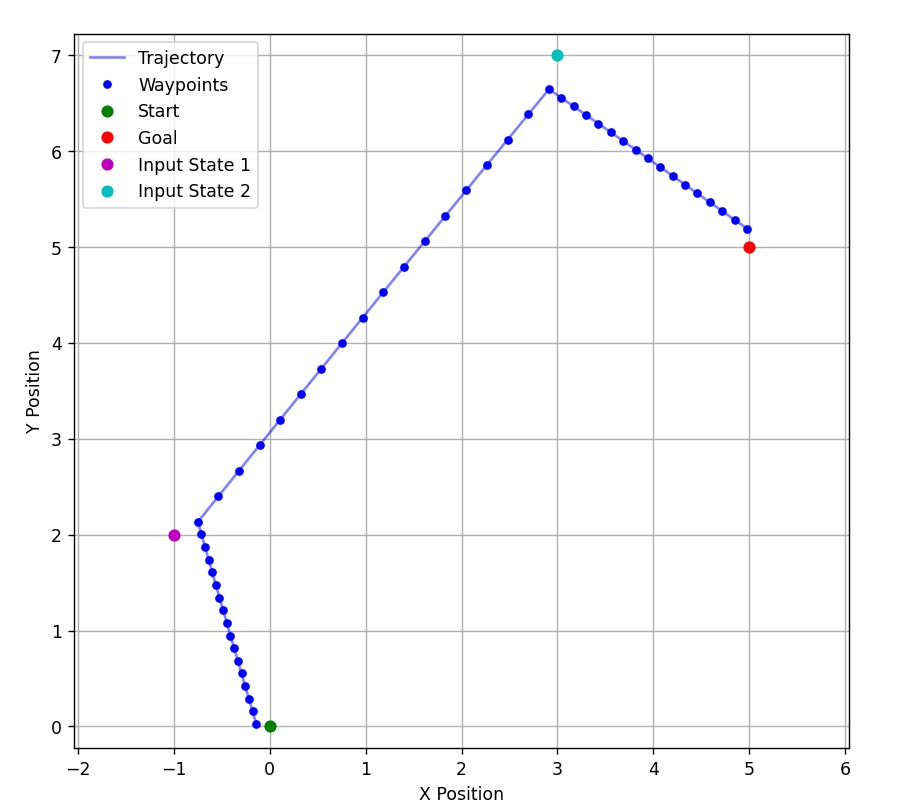
\includegraphics[width=0.5\linewidth]{latex_media/fg_traj_opt_constrained_1.jpg}
    \caption{python fg\_traj\_opt\_2.py --start 0 0 --goal 5 5 --T 50 --x0 -1 2 --x1 3 7}
    
\end{figure}

\begin{figure} [H]
    \centering
    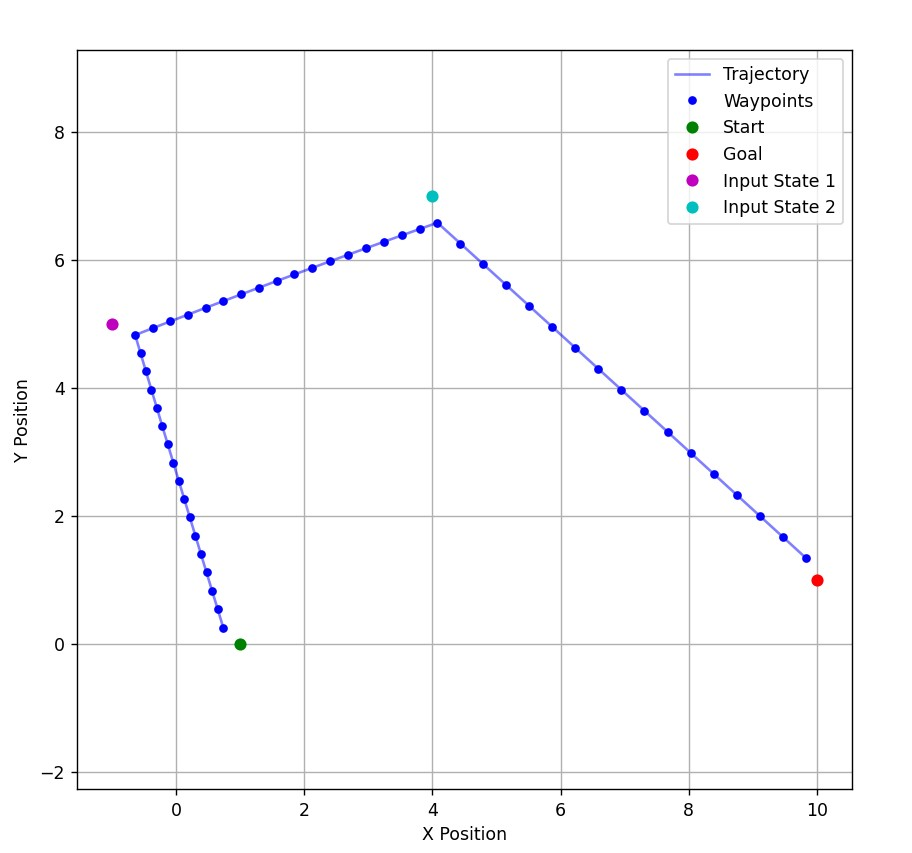
\includegraphics[width=0.5\linewidth]{latex_media/fg_traj_opt_constrained_2.jpg}
    \caption{python fg\_traj\_opt\_2.py --start 1 0 --goal 10 1 --T 50 --x0 -1 5 --x1 4 7}
    
\end{figure}

\begin{figure} [H]
    \centering
    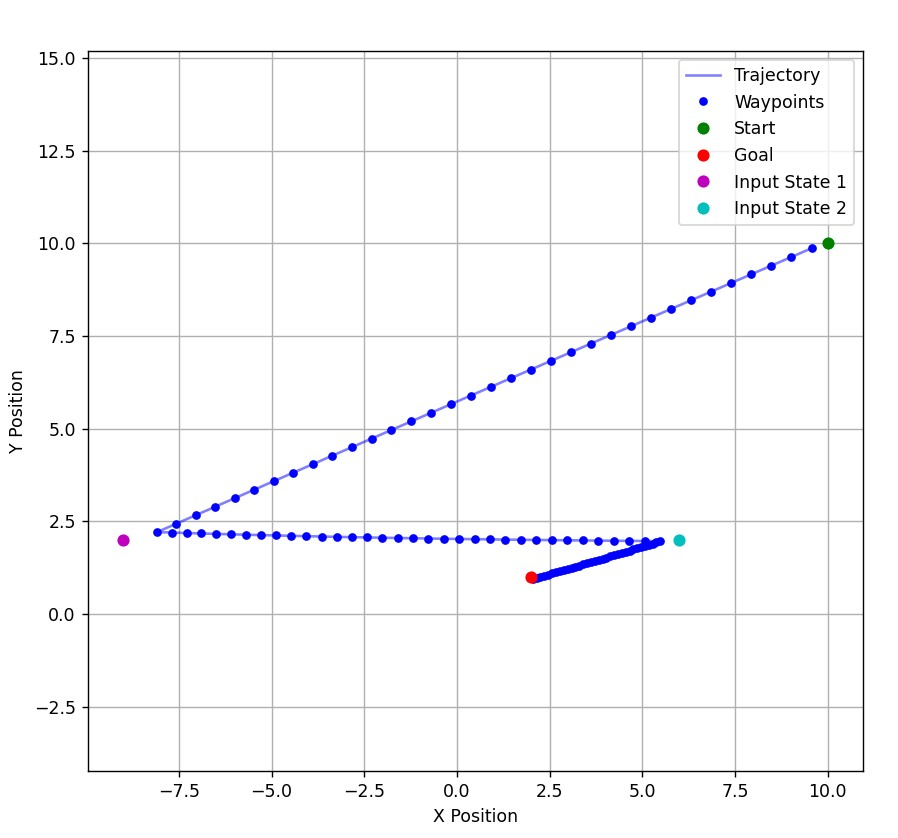
\includegraphics[width=0.5\linewidth]{latex_media/fg_traj_opt_constrained_3.jpg}
    \caption{python fg\_traj\_opt\_2.py --start 10 10 --goal 2 1 --T 100 --x0 -9 2 --x1 6 2}
    
\end{figure}


\subsection{2-Link Robot Arm}
This time we tried optimizing a 2-link arm robot. We had two joint angles instead of the x and y pose for the other robot. Our error function takes the values of theta0, theta1, u0, u1, theta0\_next, and theta1\_next and computes the predicted next states through the following equation for theta0 and theta1: $\theta^{t+1}_0 = \theta^{t}_0+(u_{0}*dt)$. We did the same for the other joint angle with its respective variables. We also started at 0 for the initial guesses, since we couldn't really interpolate here. The factor constraints remain similar to the other problems with having priors to constraint the start and goal angles and velocities, link the consecutive time steps with the dynamics equations, and the smoothness factor to ensure no major changes in velocity. Below you can see the factor graph and two visuals of the joint angles and velocities over time steps, and the end effector trajectory in the workspace in x and y coordinates.

\begin{figure} [H]
    \centering
    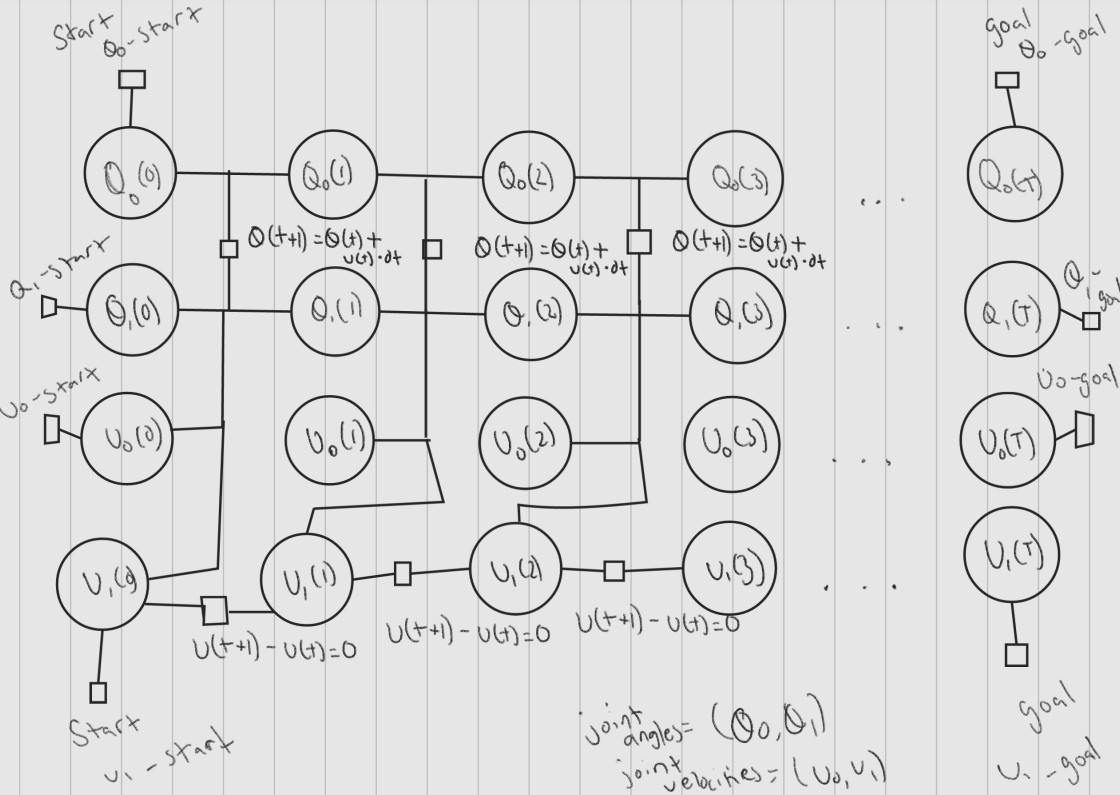
\includegraphics[width=0.5\linewidth]{latex_media/fg_traj_opt_arm_factorGraph.jpg}
    \caption{3.3 Factor Graph}
    \label{fig:enter-label}
\end{figure}

\begin{figure} [H]
    \centering
    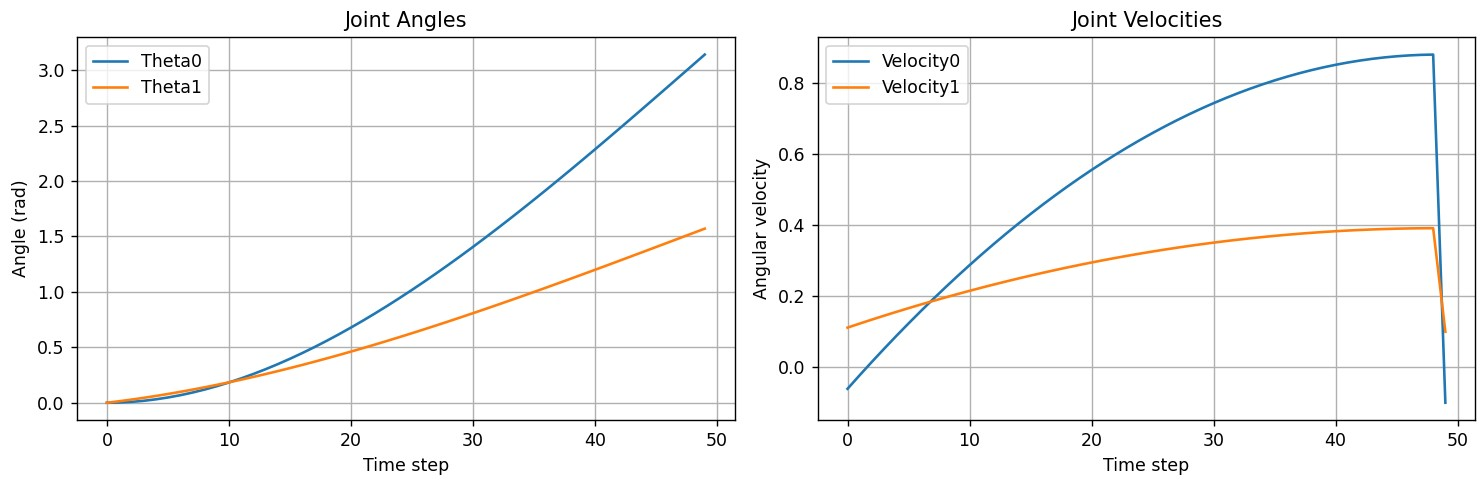
\includegraphics[width=0.5\linewidth]{latex_media/fg_traj_opt_arm_1.jpg}
    \caption{python fg\_traj\_opt\_arm.py --start 0 0 --goal 3.14 1.57 --T 50}
    \label{fig:enter-label}
\end{figure}

\begin{figure} [H]
    \centering
    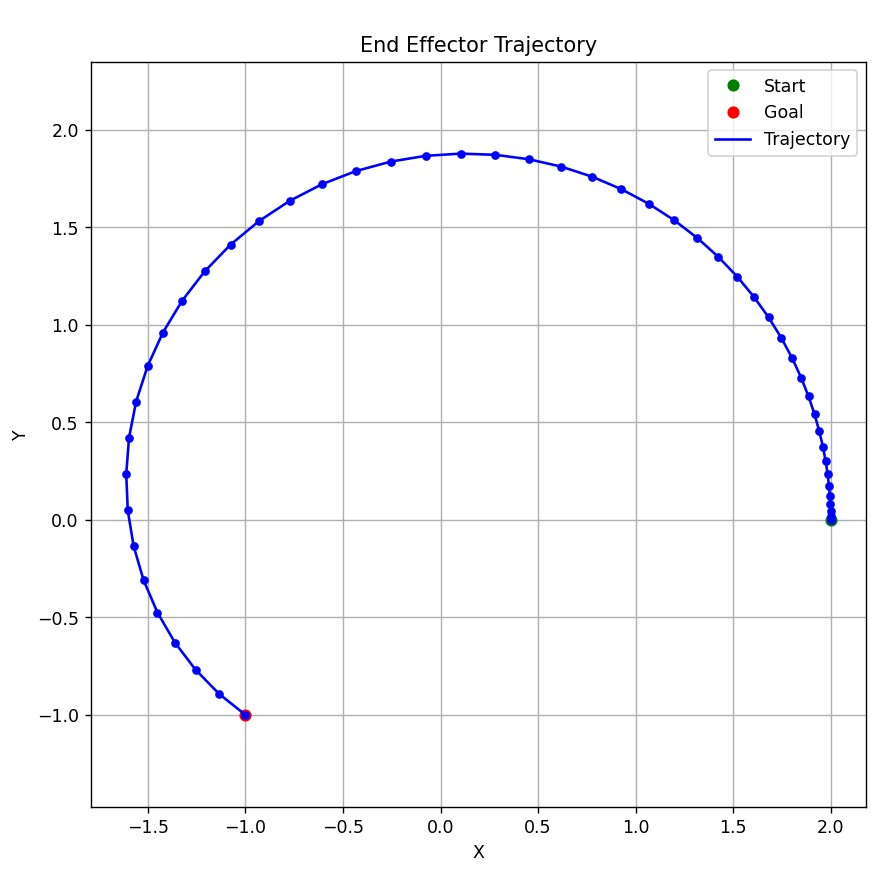
\includegraphics[width=0.5\linewidth]{latex_media/fg_traj_opt_arm_11.jpg}
    \caption{python fg\_traj\_opt\_arm.py --start 0 0 --goal 3.14 1.57 --T 50}
    \label{fig:enter-label}
\end{figure}

\begin{figure} [H]
    \centering
    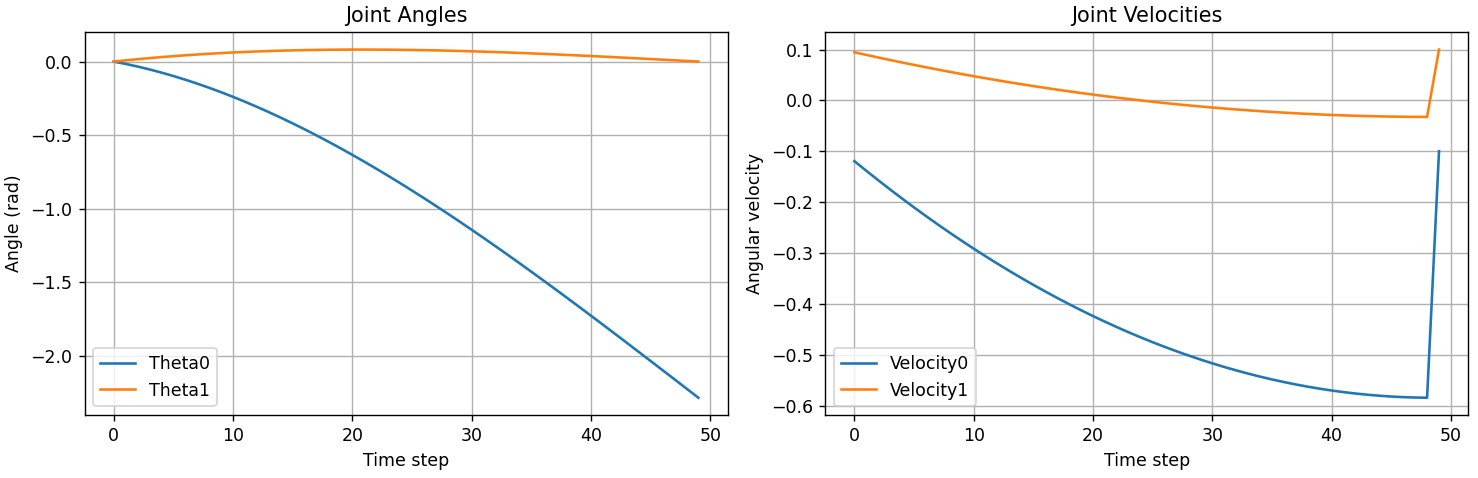
\includegraphics[width=0.5\linewidth]{latex_media/fg_traj_opt_arm_2.jpg}
    \caption{python fg\_traj\_opt\_arm.py --start 0 0 --goal 4 0 --T 50}
    \label{fig:enter-label}
\end{figure}

\begin{figure} [H]
    \centering
    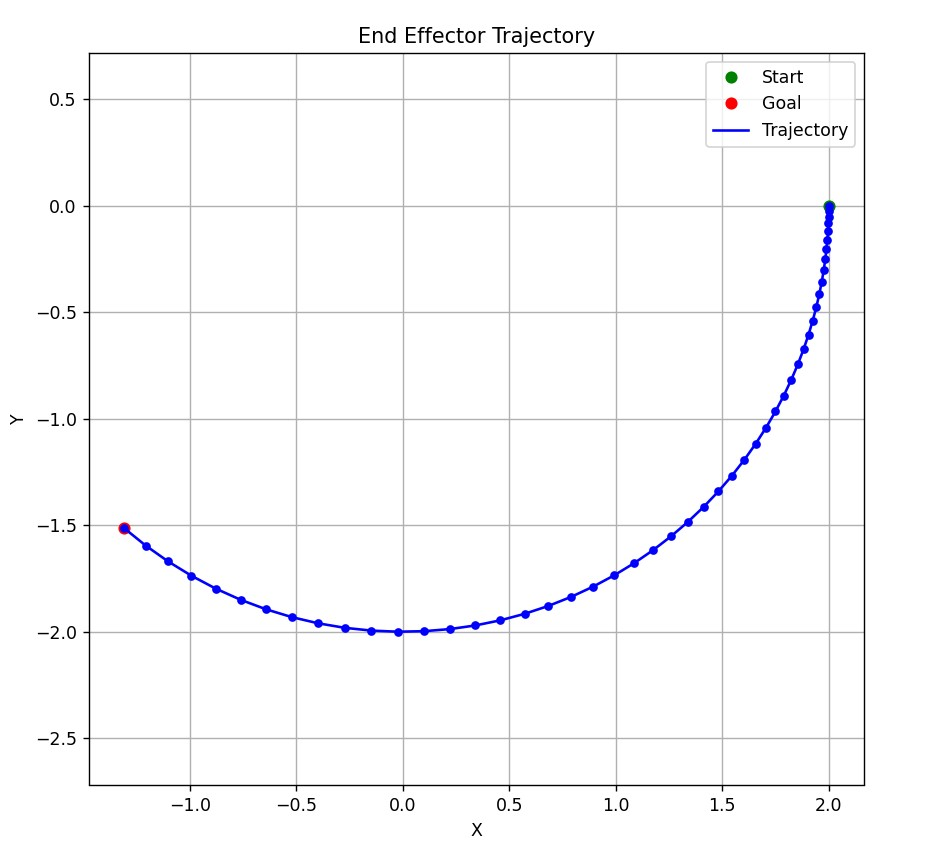
\includegraphics[width=0.5\linewidth]{latex_media/fg_traj_opt_arm_22.jpg}
    \caption{python fg\_traj\_opt\_arm.py --start 0 0 --goal 4 0 --T 50}
    \label{fig:enter-label}
\end{figure}

\begin{figure} [H]
    \centering
    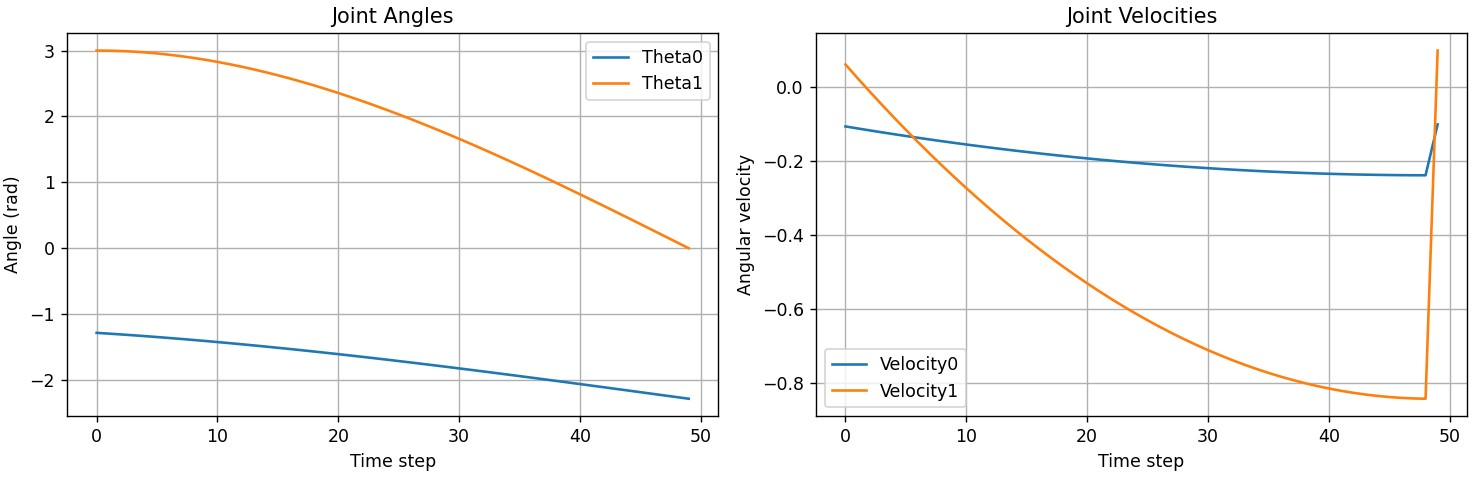
\includegraphics[width=0.5\linewidth]{latex_media/fg_traj_opt_arm_3.jpg}
    \caption{python fg\_traj\_opt\_arm.py --start 5 3 --goal 4 0 --T 50}
    \label{fig:enter-label}
\end{figure}

\begin{figure} [H]
    \centering
    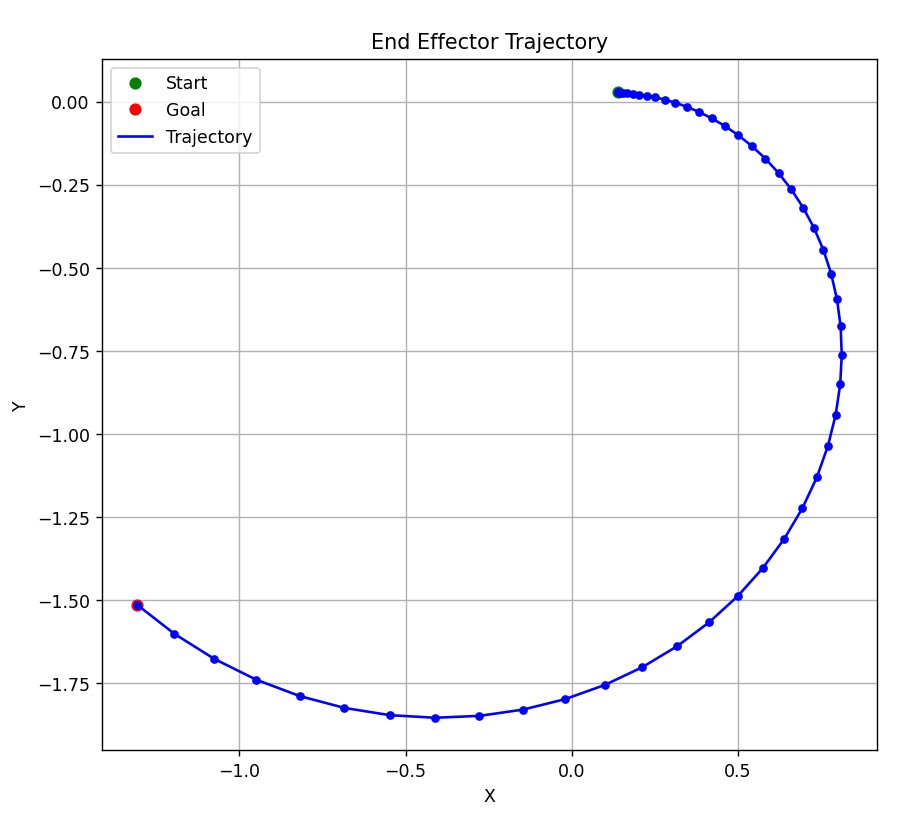
\includegraphics[width=0.5\linewidth]{latex_media/fg_traj_opt_arm_33.jpg}
    \caption{python fg\_traj\_opt\_arm.py --start 5 3 --goal 4 0 --T 50}
    \label{fig:enter-label}
\end{figure}


\section{4 Trajectory Optimization in SE(2)}
In this version of the trajectory optimization, we had to get a path for the robot in SE(2), meaning we had the addition of theta for the pose. We used GTSAM's Pose2 feature for the positions with orientation now. The error equation remains mostly the same except for the addition of theta. The Jacobians also just become 3x3 matrices now. The priors also include the theta now. The rest of the optimization stays relatively the same as SO(2).

\begin{figure} [H]
    \centering
    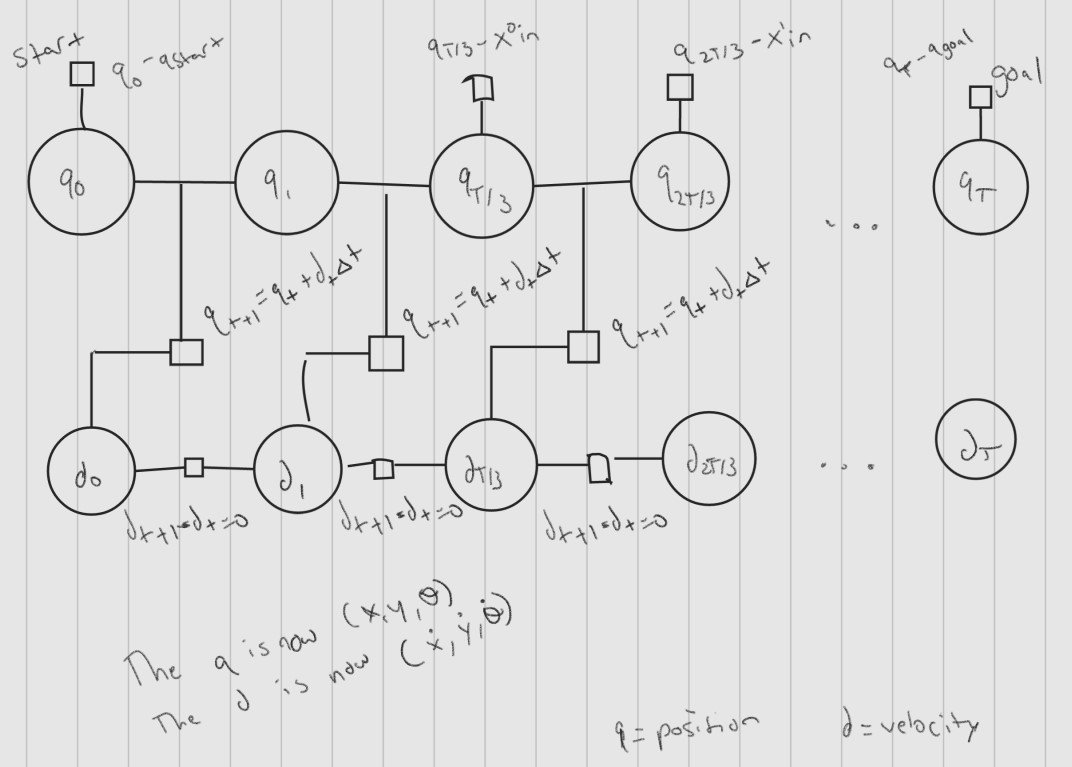
\includegraphics[width=0.5\linewidth]{latex_media/fg_traj_opt_se2_factorGraph.jpg}
    \caption{4 Factor Graph}
    \label{fig:enter-label}
\end{figure}

\begin{figure} [H]
    \centering
    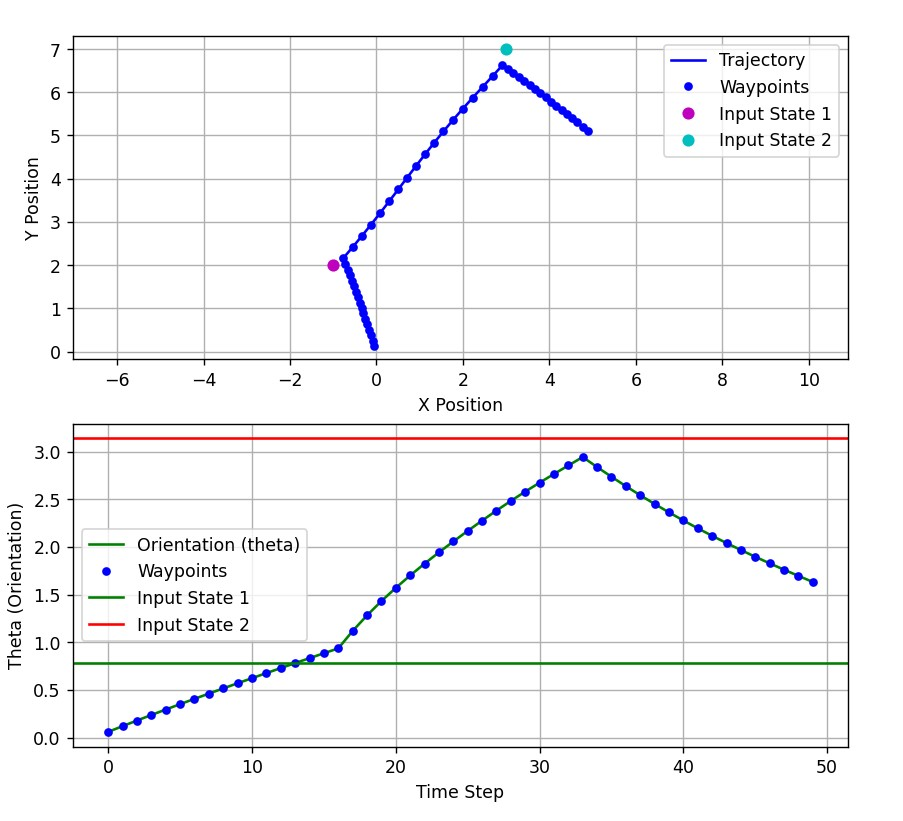
\includegraphics[width=0.5\linewidth]{latex_media/fg_traj_opt_se2_1.jpg}
    \caption{python fg\_traj\_opt\_se2.py --start 0 0 0 --goal 5 5 1.57 --T 50 --x0 -1 2 0.78 --x1 3 7 3.14}
\end{figure}

\begin{figure} [H]
    \centering
    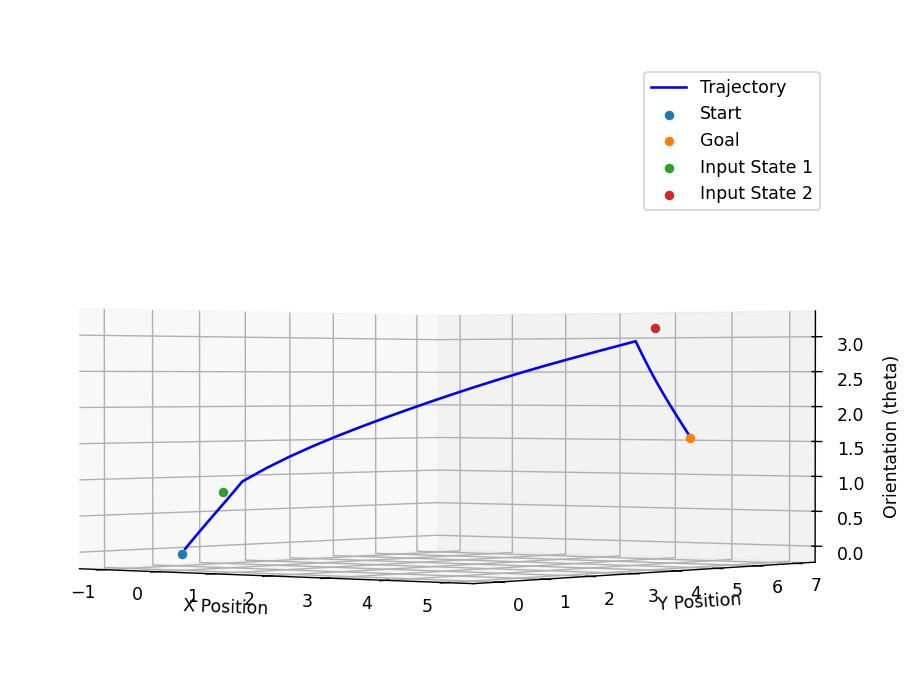
\includegraphics[width=0.5\linewidth]{latex_media/fg_traj_opt_se2_11.jpg}
    \caption{python fg\_traj\_opt\_se2.py --start 0 0 0 --goal 5 5 1.57 --T 50 --x0 -1 2 0.78 --x1 3 7 3.14}
    
\end{figure}

\begin{figure} [H]
    \centering
    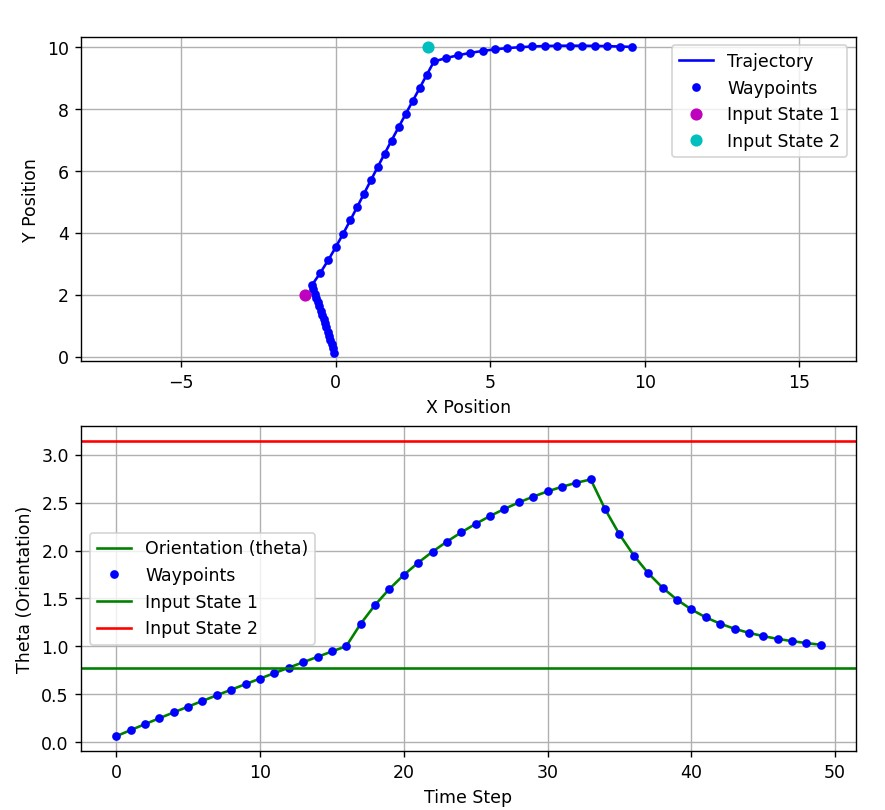
\includegraphics[width=0.5\linewidth]{latex_media/fg_traj_opt_se2_2.jpg}
    \caption{python fg\_traj\_opt\_se2.py --start 0 0 0 --goal 10 10 1 --T 50 --x0 -1 2 0.78 --x1 3 10 3.14}
    
\end{figure}

\begin{figure} [H]
    \centering
    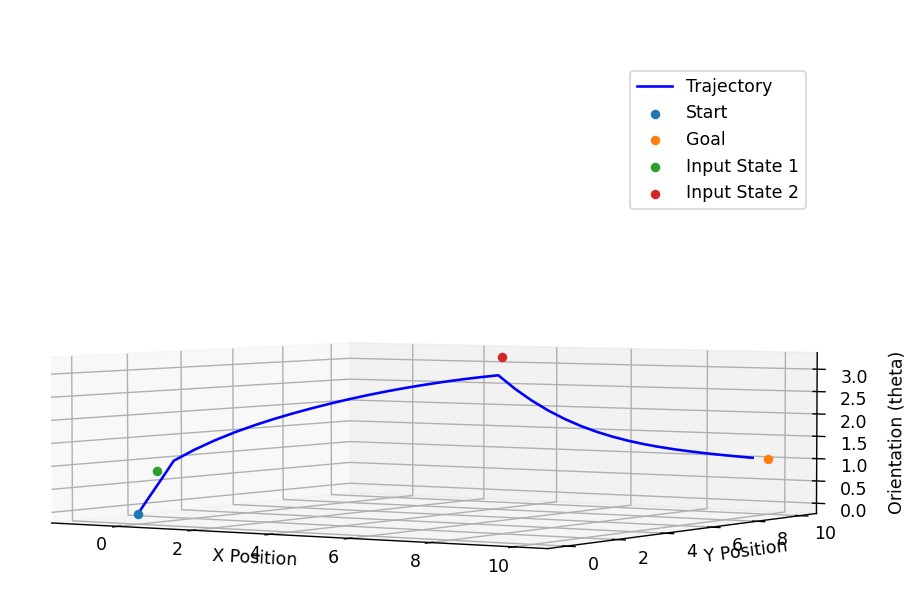
\includegraphics[width=0.5\linewidth]{latex_media/fg_traj_opt_se2_22.jpg}
    \caption{python fg\_traj\_opt\_se2.py --start 0 0 0 --goal 10 10 1 --T 50 --x0 -1 2 0.78 --x1 3 10 3.14}
    
\end{figure}

\begin{figure} [H]
    \centering
    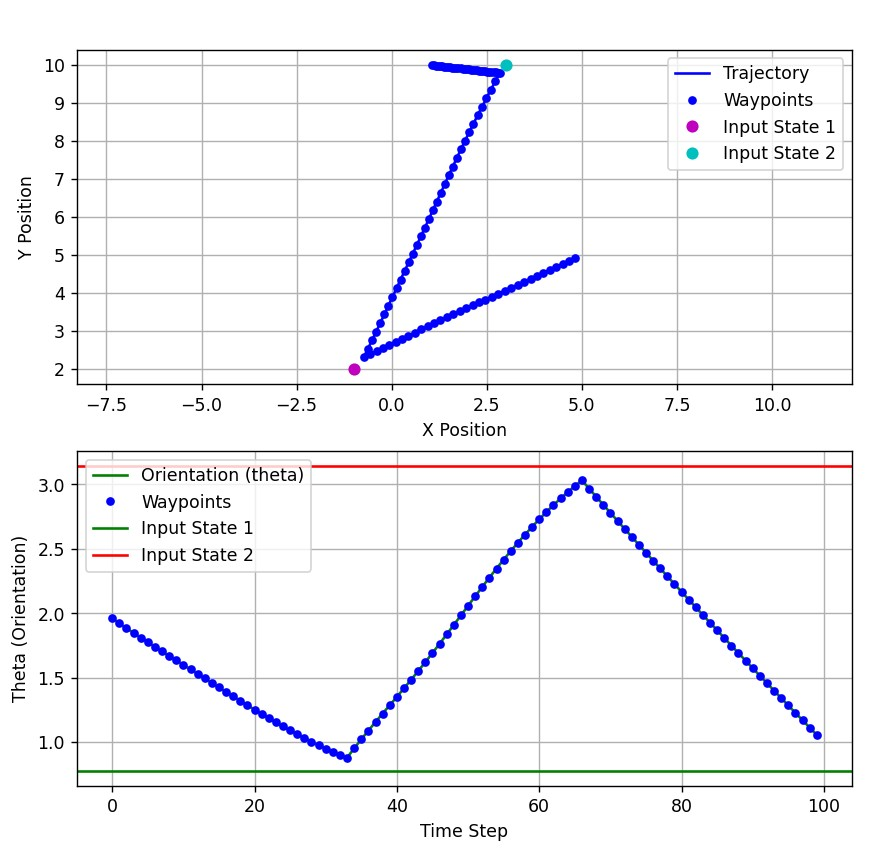
\includegraphics[width=0.5\linewidth]{latex_media/fg_traj_opt_se2_3.jpg}
    \caption{ python fg\_traj\_opt\_se2.py --start 5 5 2 --goal 1 10 1 --T 100 --x0 -1 2 0.78 --x1 3 10 3.14}
    
\end{figure}

\begin{figure} [H]
    \centering
    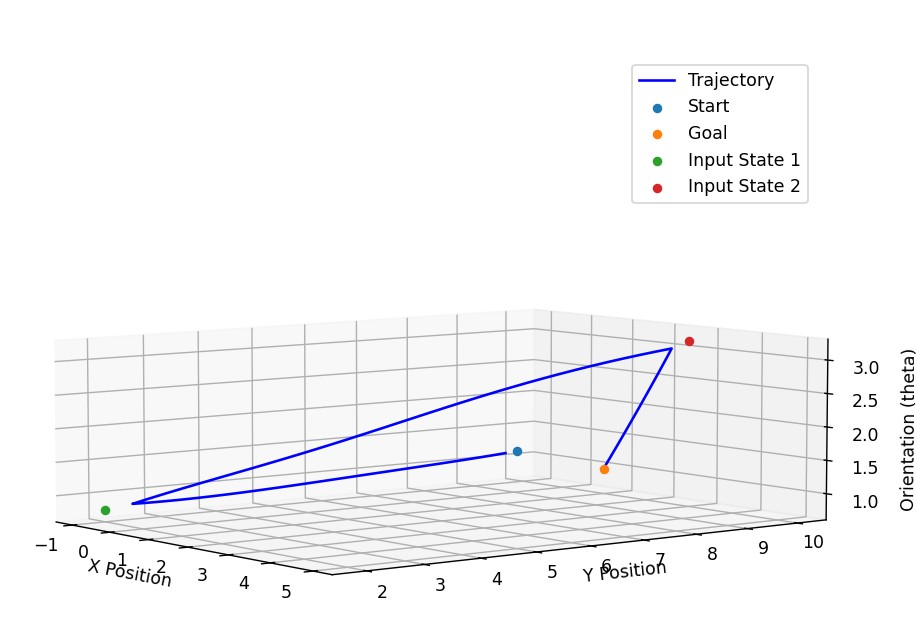
\includegraphics[width=0.5\linewidth]{latex_media/fg_traj_opt_se2_33.jpg}
    \caption{ python fg\_traj\_opt\_se2.py --start 5 5 2 --goal 1 10 1 --T 100 --x0 -1 2 0.78 --x1 3 10 3.14}
    
\end{figure}

\end{document}